% 
% Annual Cognitive Science Conference
% Sample LaTeX Paper -- Proceedings Format
% 

% Original : Ashwin Ram (ashwin@cc.gatech.edu)       04/01/1994
% Modified : Johanna Moore (jmoore@cs.pitt.edu)      03/17/1995
% Modified : David Noelle (noelle@ucsd.edu)          03/15/1996
% Modified : Pat Langley (langley@cs.stanford.edu)   01/26/1997
% Latex2e corrections by Ramin Charles Nakisa        01/28/1997 
% Modified : Tina Eliassi-Rad (eliassi@cs.wisc.edu)  01/31/1998
% Modified : Trisha Yannuzzi (trisha@ircs.upenn.edu) 12/28/1999 (in process)
% Modified : Mary Ellen Foster (M.E.Foster@ed.ac.uk) 12/11/2000
% Modified : Ken Forbus                              01/23/2004
% Modified : Eli M. Silk (esilk@pitt.edu)            05/24/2005
% Modified : Niels Taatgen (taatgen@cmu.edu)         10/24/2006
% Modified : David Noelle (dnoelle@ucmerced.edu)     11/19/2014
% Modified : Roger Levy (rplevy@mit.edu)     12/31/2018



%% Change "letterpaper" in the following line to "a4paper" if you must.

\documentclass[10pt,letterpaper]{article}

\usepackage{cogsci}

\cogscifinalcopy % Uncomment this line for the final submission 


\usepackage{pslatex}
\usepackage{apacite}
\usepackage{float} % Roger Levy added this and changed figure/table
                   % placement to [H] for conformity to Word template,
                   % though floating tables and figures to top is
                   % still generally recommended!

%\usepackage[none]{hyphenat} % Sometimes it can be useful to turn off
%hyphenation for purposes such as spell checking of the resulting
%PDF.  Uncomment this block to turn off hyphenation.

% custom packages
\usepackage{graphicx}
\usepackage{adjustbox}
\usepackage{subcaption}
\usepackage{url}
\urlstyle{same}

%\setlength\titlebox{4.5cm}
% You can expand the titlebox if you need extra space
% to show all the authors. Please do not make the titlebox
% smaller than 4.5cm (the original size).
%%If you do, we reserve the right to require you to change it back in
%%the camera-ready version, which could interfere with the timely
%%appearance of your paper in the Proceedings.



\title{The Effect of State Representations in Sequential Sensory Prediction: Introducing the Shape Sequence Task}
 
\author{{\large \bf Henrik Siljebråt (h.siljebrat@gold.ac.uk)} \\
  Department of Computing, Goldsmiths, University of London
  \AND {\large \bf Alan Pickering (a.pickering@gold.ac.uk)} \\
  Department of Psychology, Goldsmiths, University of London}


\begin{document}

\maketitle


\begin{abstract}
How do humans learn models supporting decision making? Reinforcement learning (RL) is a success story both in artificial intelligence and neuroscience. Essential to these RL models are state representations. Based on what current state an animal or artificial agent is in, they learn optimal actions by maximizing future expected reward. But how are humans able to learn and create representations of states? We introduce a novel sequence prediction task with hidden structure where participants have to combine learning and memory to find the proper state representation, without the task explicitly indicating such structure. We show that humans are able to find this pattern, while a sensory prediction error version of RL cannot, unless equipped with appropriate state representations. Furthermore, in slight variations of the task, making it more difficult for humans, the RL-derived model with simple state representations sufficiently describes behaviour and suggests that humans fall back on simple state representations when a more optimal task representation cannot be found. We argue this task allows to investigate previously proposed models of state and task representations as well as supporting recent results indicating that RL describes a more general sensory prediction error function for dopamine, rather than predictions focussed solely on reward.

\textbf{Keywords:} 
reinforcement learning; state representation; sensory prediction error; computational modelling; human experiment
\end{abstract}


The theory of reinforcement learning (RL) is a success story, both in artificial intelligence and neuroscience. When sufficiently scaled up, artificial RL systems can learn to play board games such as \emph{Chess} and \emph{Go} \cite{Silver2018-gk} as well as video games like \emph{Dota 2} \cite{OpenAI2019-xb}. RL algorithms also appear to describe accurately how dopamine systems in mammalian brains use reward prediction errors (RPEs) to learn \cite{Schultz2015-oz}. Positive RPEs are generated by bigger rewards than expected, while smaller than expected rewards generate negative RPEs. These errors are reflected in the phasic \cite{Schultz2016-ul} increases or decreases in dopamine cell firing, respectively.

RL is a mathematical formalization of learning built on foundational work by Rescorla and Wagner \citeyear{Rescorla1972-na} combined with Markov Decision Processes \cite{Sutton2018-an}. In essence, RL has four parts; states, actions, rewards and the state transition function, describing how one state follows another. With the goal of maximizing reward, an agent, biological or artificial, moves through a world compartmentalized into states, where each state has a set of possible actions. By selecting actions, the state transitions to the next, the agent receives some reward (or none) and is now ready to select a new action. Through trial-and-error the agent learns to associate each state-action pair with a value and can thus learn to optimize its behaviour. Importantly, for these algorithms to work, they rely on the Markov property (the agent does not need to rely on explicit memory of previous experiences); all information to select the optimal path is contained in the current state and action values.

Previous research often take states for granted  \cite{Niv2019-xg}. In computerised experimental tasks, a state is the idealized representation of what the participant sees on the monitor and in machine learning the state is usually a vector of pixels. In real world situations, however, observations are high-dimensional and continuous. This means there is often the need to (1) generalize between states that look different but are actually similar and/or (2) differentiate between states that look the same but are actually different. Real world observations also often do not have enough information to adhere to the Markov property since many situations require memory of previous events or inference of hidden causes. Furthermore, most RL algorithms converge (find the optimum) for certain only when all states and actions have been visited an infinite number of times \cite{Sutton2018-an}. Biological organisms cannot possibly try every possible sequence of actions.

Generalising RL in artificial intelligence research has proved difficult \cite{Justesen2018-um}, as systems are optimized for specific tasks and training on new tasks can lead to so called catastrophic forgetting \cite{Kirkpatrick2017-vk}. In spite of this, machine learning systems based mainly on RL work surprisingly well for game playing when scaled up \cite{OpenAI2019-xb}, because they use massive amounts of data and computational resources. By contrast, animals can represent states in a way that proves more efficient; this ability probably involves interaction between many systems \cite{Collins2019-of, Niv2019-xg}. Generalization may involve attentional processes \cite{Niv2019-xg} that reduce observational complexity, and by inferring hidden (latent) structure \cite{Gershman2010-oc} generalization and differentiation may work together to cluster experiences, forming belief state distributions \cite{Schuck2018-ik,Starkweather2017-yj}. In practice this could work by constructing task-sets (rules) that differ depending on context \cite{Collins2013-cv}, perhaps supported by processes such as working memory \cite{Collins2018-ga} and episodic memory \cite{Gershman2017-ah}.

\subsection{Representations and models}
The classic view of how simple associations between states and actions are supported by internal models of task structure can be found in the distinction between the two main variants of RL; model-based (MB) and model-free (MF) \cite{Daw2005-ti,Doll2012-ou}. Both variants are updated based on experience of the world, but where MF approaches work by saving state-values similar to a spreadsheet, MB algorithms also learn the state transition function and thus predict values of actions by simulating the future. Importantly, if the goal and/or reward function changes, MF algorithms have to relearn from scratch whereas MB algorithms are more flexible.

These two systems appear to be intermixed to such a degree in the brain that separation is difficult \cite{Doll2012-ou,Schultz2016-ul,Simon2011-mg,Tsutsui2016-iq}. Recent work has proposed different solutions such as rethinking what model-based means \cite{Langdon2018-jh}, or combining MB and MF into an intermediate "successor representation" \cite{Momennejad2020-lk}. Building on the latter is the “sensory prediction error” (SPE) hypothesis of dopamine \cite{Gardner2018-vj}, suggesting dopamine cell firing codes for more aspects than just reward.

A hierarchical approach might be useful; to frame the two systems as top-down versus bottom-up, where top-down predictions from a world model are compared and/or integrated with bottom-up incoming sensory information. This view forms the basis of theories of predictive coding \cite{Clark2013-hr} and free energy \cite{Friston2010-wi} and would appear to fit with evidence for both model-free and model-based predictions at many different levels of dopamine function \cite{Doll2012-ou}. Other hierarchical proposals add richer state representations to RL \cite{Langdon2018-jh}, or use machine learning systems where MF trains MB \cite{Botvinick2019-qf}, or emphasize how working memory seems to influence RL prediction error \cite{Collins2018-ga}.

However, even armed with this framing, it is not clear how interacting with a task leads to changing state representations depending on the (latent) task structure, although some accounts show promise \cite{Eckstein2020-yi}. We therefore aimed to create a task able to probe this, while being as simple as possible to reduce instructional needs. We also wanted to investigate whether RL based on sensory prediction errors could describe behaviour in the absence of explicit rewards \cite{Gershman2013-bo,gershman2014statistical}, and also illustrate how changing the coding of state representations for such RL models would impact the performance of our models. Our main contribution here is thus to introduce our novel task, which we believe will offer an important test-bed for the more complex approaches to RL listed above.

\begin{figure}[t]
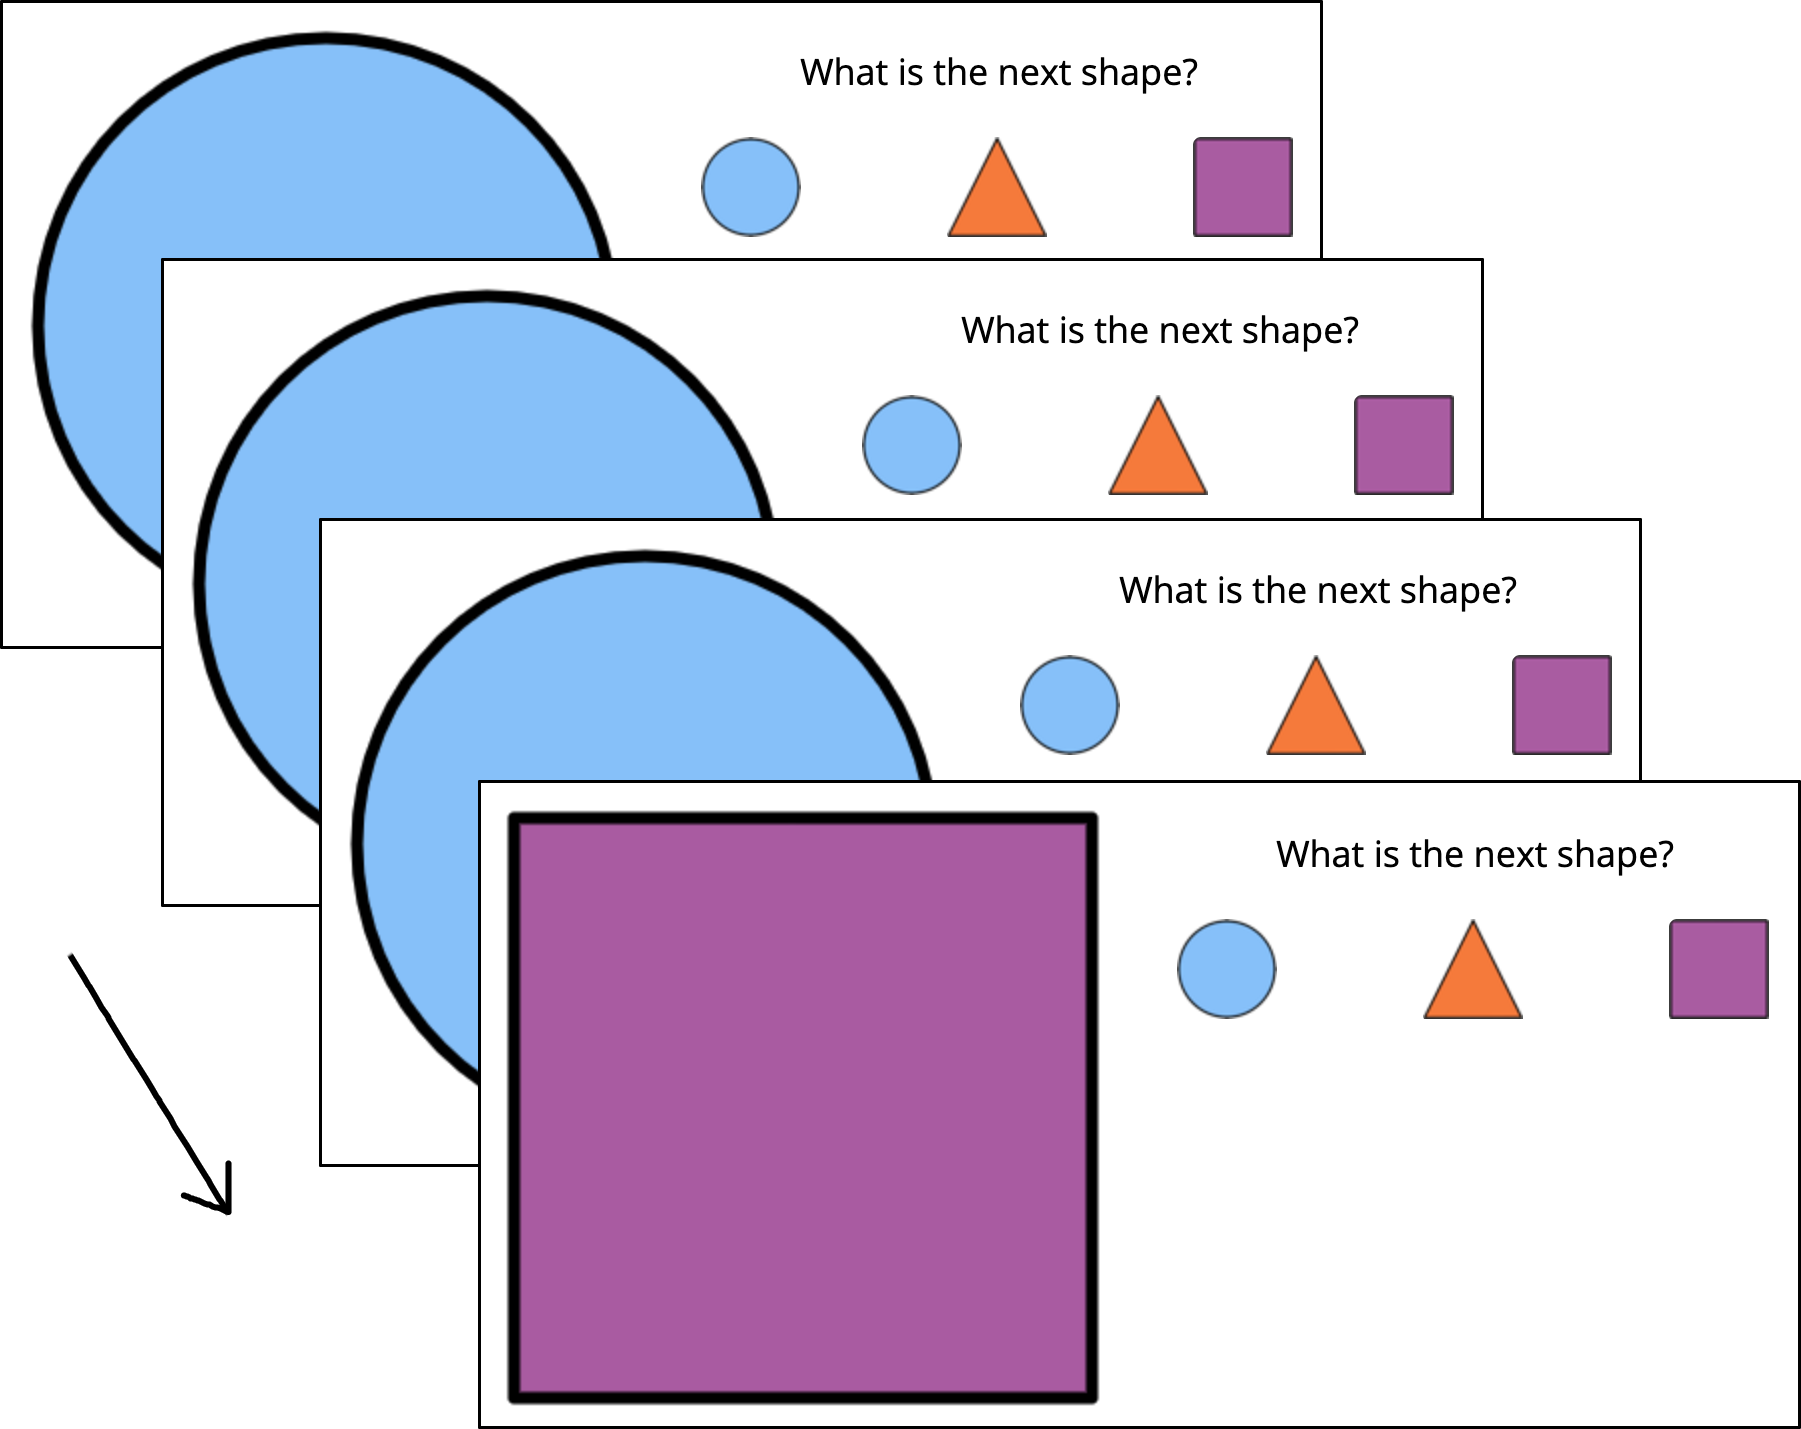
\includegraphics[width=0.45\textwidth]{new_task_sequence.png}
\caption{Task setup. The participant sees a large shape on the screen, and three options for what shape they think will come next. The choice options are always presented in the same spatial arrangement. When the participant has clicked, the next shape appears, meaning the only feedback is the next stimulus itself. In all experiments, shapes mainly repeat three times in a row. However, the sequence of shapes depends on experiment variant as explained in the text. Picture shown is the task as presented in Experiments B-D.}
\centering
\label{fig:figure1}
\end{figure}

\subsection{The sequential shape task}
The task is deceptively simple; participants see a large colored shape on screen, together with three options for what shape they think will come next (Figure 1). The possible shapes are blue circle, orange triangle, and purple square and the response option buttons are small versions of the same shapes. The options are always presented in the same order. The participant indicates their choice by clicking one of the buttons and the next shape in the sequence appears.

The sequential patterns can be conceptualised by imagining three bags, where each bag has three shapes of the same kind inside. All the shapes in one bag are drawn before shapes from another bag are drawn\footnote{This idea of bags of shapes is simply to understand the task properties and is not mentioned to participants.}. Thus, the underlying basic pattern is that each shape will be presented three times in a row. As we explain below, there are 3 task variants which vary in how the next bag of shapes is drawn after the current bag is emptied.

The task is thus able to investigate the influence of higher-order hidden state properties (what ‘bag’ are we in currently) as well as the process of going from states as single trials (one shape) to states as several trials (bag). More importantly, it can investigate differentiation of states (as discussed above), since all trial screens within the same bag look the same, but the third repeat of a shape may require a different response, as the latent context is now ‘last shape before next bag’.

\section{Methods}

We used three different versions of the shape sequence task. In all versions imagine that, after a bag is emptied of its 3 shapes, it is refilled. The first version (“random”) selects the next bag at random, so that after a sequence of three shapes of one kind, the probability was 1/3 that the next bag selected would contain the same shape as the previous bag. Over the duration of the task, we might therefore expect participants to learn this pattern of  ‘shifts’ in shape type (about 2/3 of the runs of the same shape will be of length 3 and then a shift). However, since bags are drawn at random there is a fairly large chance that the same shape will appear in runs of 6 (about 22\% of the time) or 9 (about 7.5\% of the time) in a row, and so the shape shifts will occur after varying multiples of 3 trials and thus will be hard to predict.

The second version we call ‘bag of bags’ (bob), as we imagine a large bag with three smaller bags in it. The small bags are drawn randomly, without replacement, until the large bag is empty. This means that a particular bag of shapes cannot be re-used until the other two bags have been used. Thus, shape shifts occur after a sequence of 3 repeats with an expected probability of 0.89 and 6 times in a row with an expected probability of 0.11. Predicting the shifts is thus expected to still be difficult for human participants, but somewhat easier than for the random version.

The third version of the task we call ‘bag of bags without repeat’ (bob-wr). It is basically the same as the ‘bob’ version, with the additional constraint that when drawing the first small bag after returning all 3 bags to the ‘bag of bags’, it must differ from the last small bag used. In other words, the same shape can be shown a maximum of three times in a row. We predicted this would be the easiest version for participants.

Although these 3 versions of the task were expected to elicit differential shift prediction behaviour in human participants, analysis and preliminary simulations led us to predict that our basic RL model (see simulations section below) would learn all 3 versions of the task in a similar way. This prediction was based on using a state coding for the task in which each shape was coded using a vector of 3 bits with one bit coding the presence of a specific shape on each trial.

\subsection{Experiments}

Experiment A had a total of 270 trials, or 90 bags, taking around 10-15 minutes. In this experiment, considered a pilot study, we had only the circle shape and instead used different colors to differentiate bags. For Experiment B-D there were 99 trials, or 33 bags, for an average run time of 5 minutes. Here we had three different shapes; circle, triangle and square, and each shape was also differentiated by being of a different but consistent color. Experiment B-D (as in Figure 1) also included a slight delay of one second for the choice options to appear, in order to discourage participants clicking through the experiment without effort. Participants in Experiment B-D were excluded from final analysis if they had an average response time below one second or left the experiment window for more than 30 seconds in total during the experiment. Experiment B-D also included a free text entry at the end asking if the participant had spotted a pattern.

Experiment A: 27 people were recruited via Amazon Mechanical Turk. They were paid approximately £10/h for participating, and we set a condition that they had to have at least 100 previously approved submissions to Amazon Mechanical Turk to participate. They did the random version of the task, with the same fixed random sequence for all participants determined by a single random seed. In this random sequence there were 45 sequences of 3 identical shapes in a row, 16 of 6 in a row, 3 of 9 in a row and 1 of 12.

Experiment B: 39 people (mean age 28 (SD 8), 18 females) were recruited for the bob-wr version of the task via Prolific, of which 7 had to be excluded.

Experiment C: 40 people (mean age 28 (SD 9), 17 females) were recruited for the bob version of the task via Prolific, of which 2 had to be excluded.

Experiment D: 40 people (mean age 30 (SD 11), 18 females) were recruited for the random version of the task via Prolific, of which 1 had to be excluded. 

In B to D, seeds were randomized, meaning that a unique random sequence (subject to the constraints of the different versions) was used for each participant.

\subsubsection{Scoring} If the prediction on the previous trial was correct, and the prediction on the current trial matched that of previous trial it was scored as win-stay. If the prediction of the previous trial was wrong, and the prediction on the current trial was different from the previous prediction, it counted as lose-shift. Additionally we scored a “shift prediction” whenever the prediction of the next shape was different from the current shape. Finally, we scored for accuracy, i.e. when the prediction of the next shape was correct. All scores were each calculated for every trial.

\subsubsection{Code availability} Code for the experiment, results (including graphs not shown here) and simulations can be found at \url{https://github.com/fohria/cogsci2020}

% expA and simA results

\begin{figure*}[t]
\centering
\captionsetup{justification=centering}

\begin{subfigure}{0.33\textwidth}
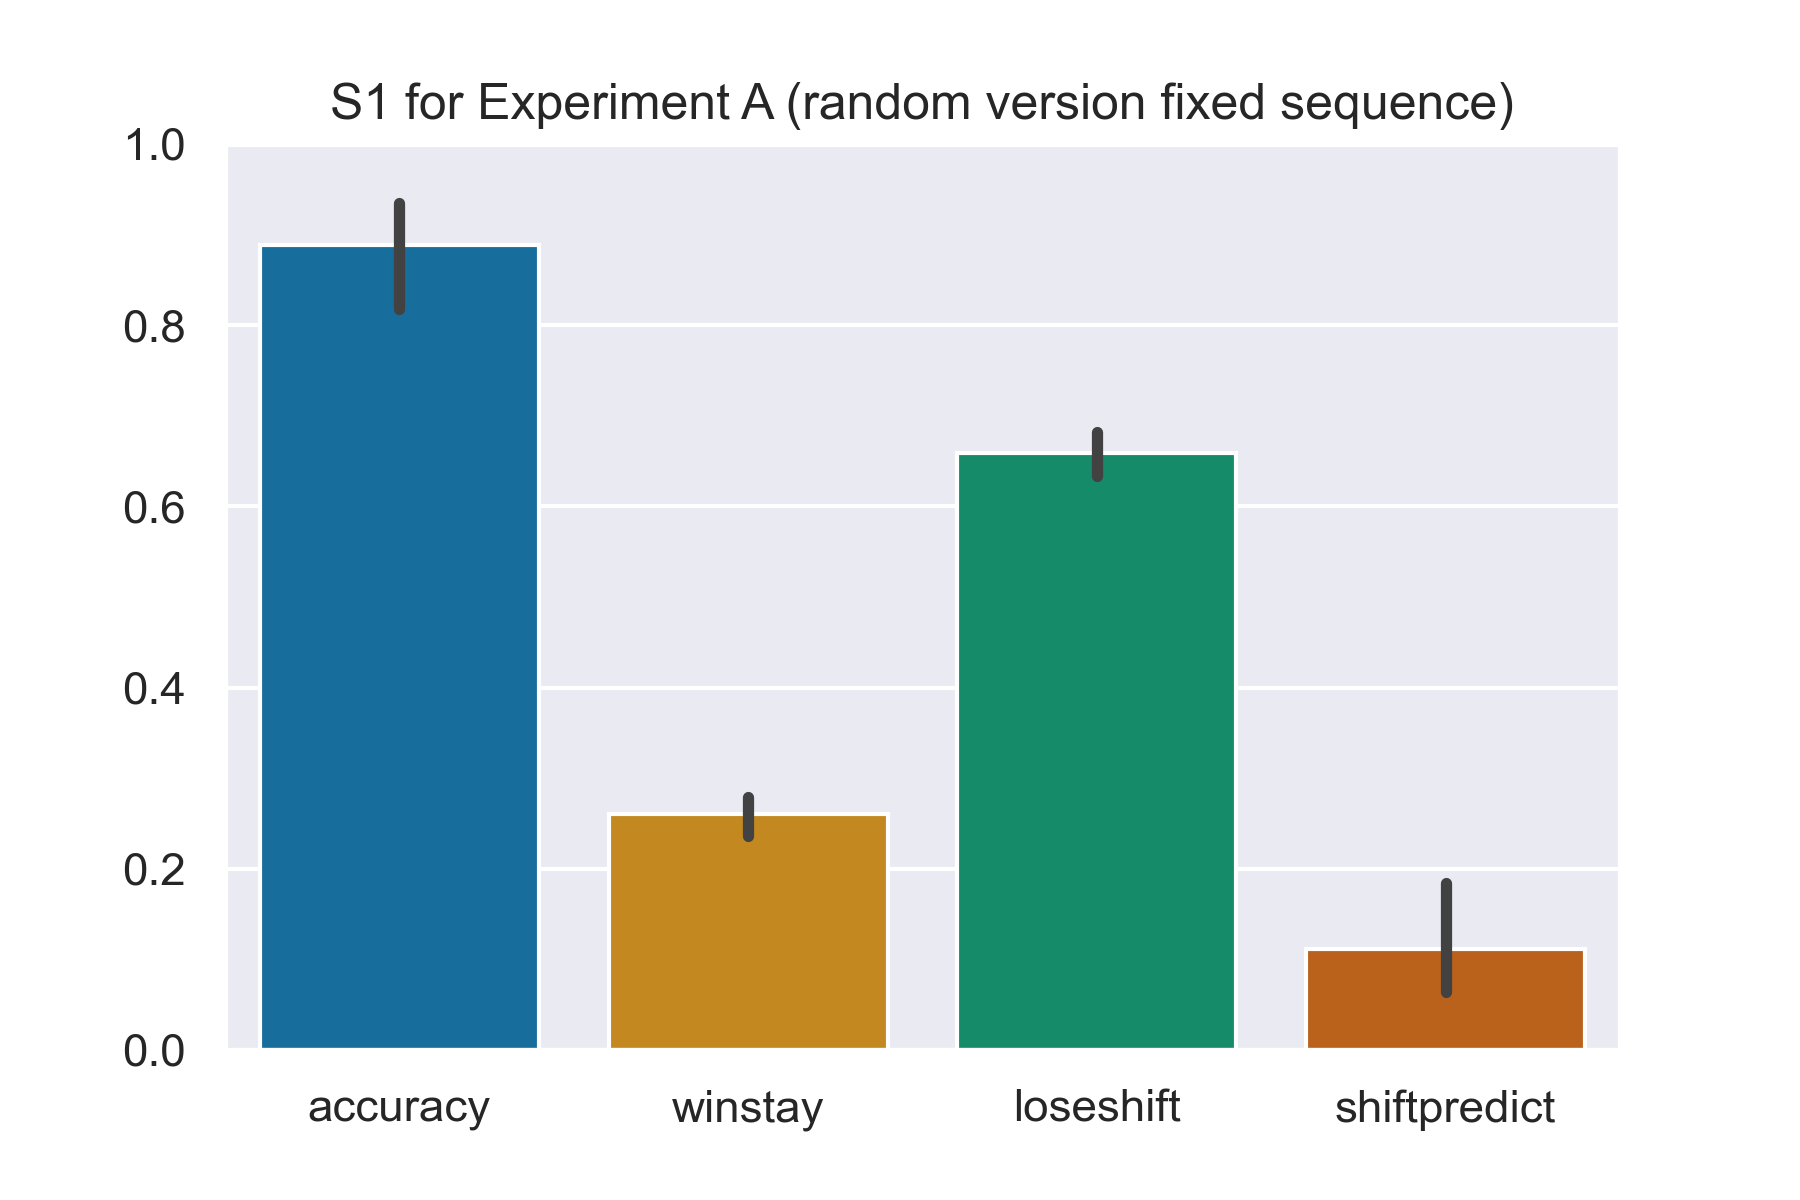
\includegraphics[width=0.9\linewidth, height=4cm]{plots/expA_s1.png} 
\label{fig:expA1}
\end{subfigure}
\begin{subfigure}{0.33\textwidth}
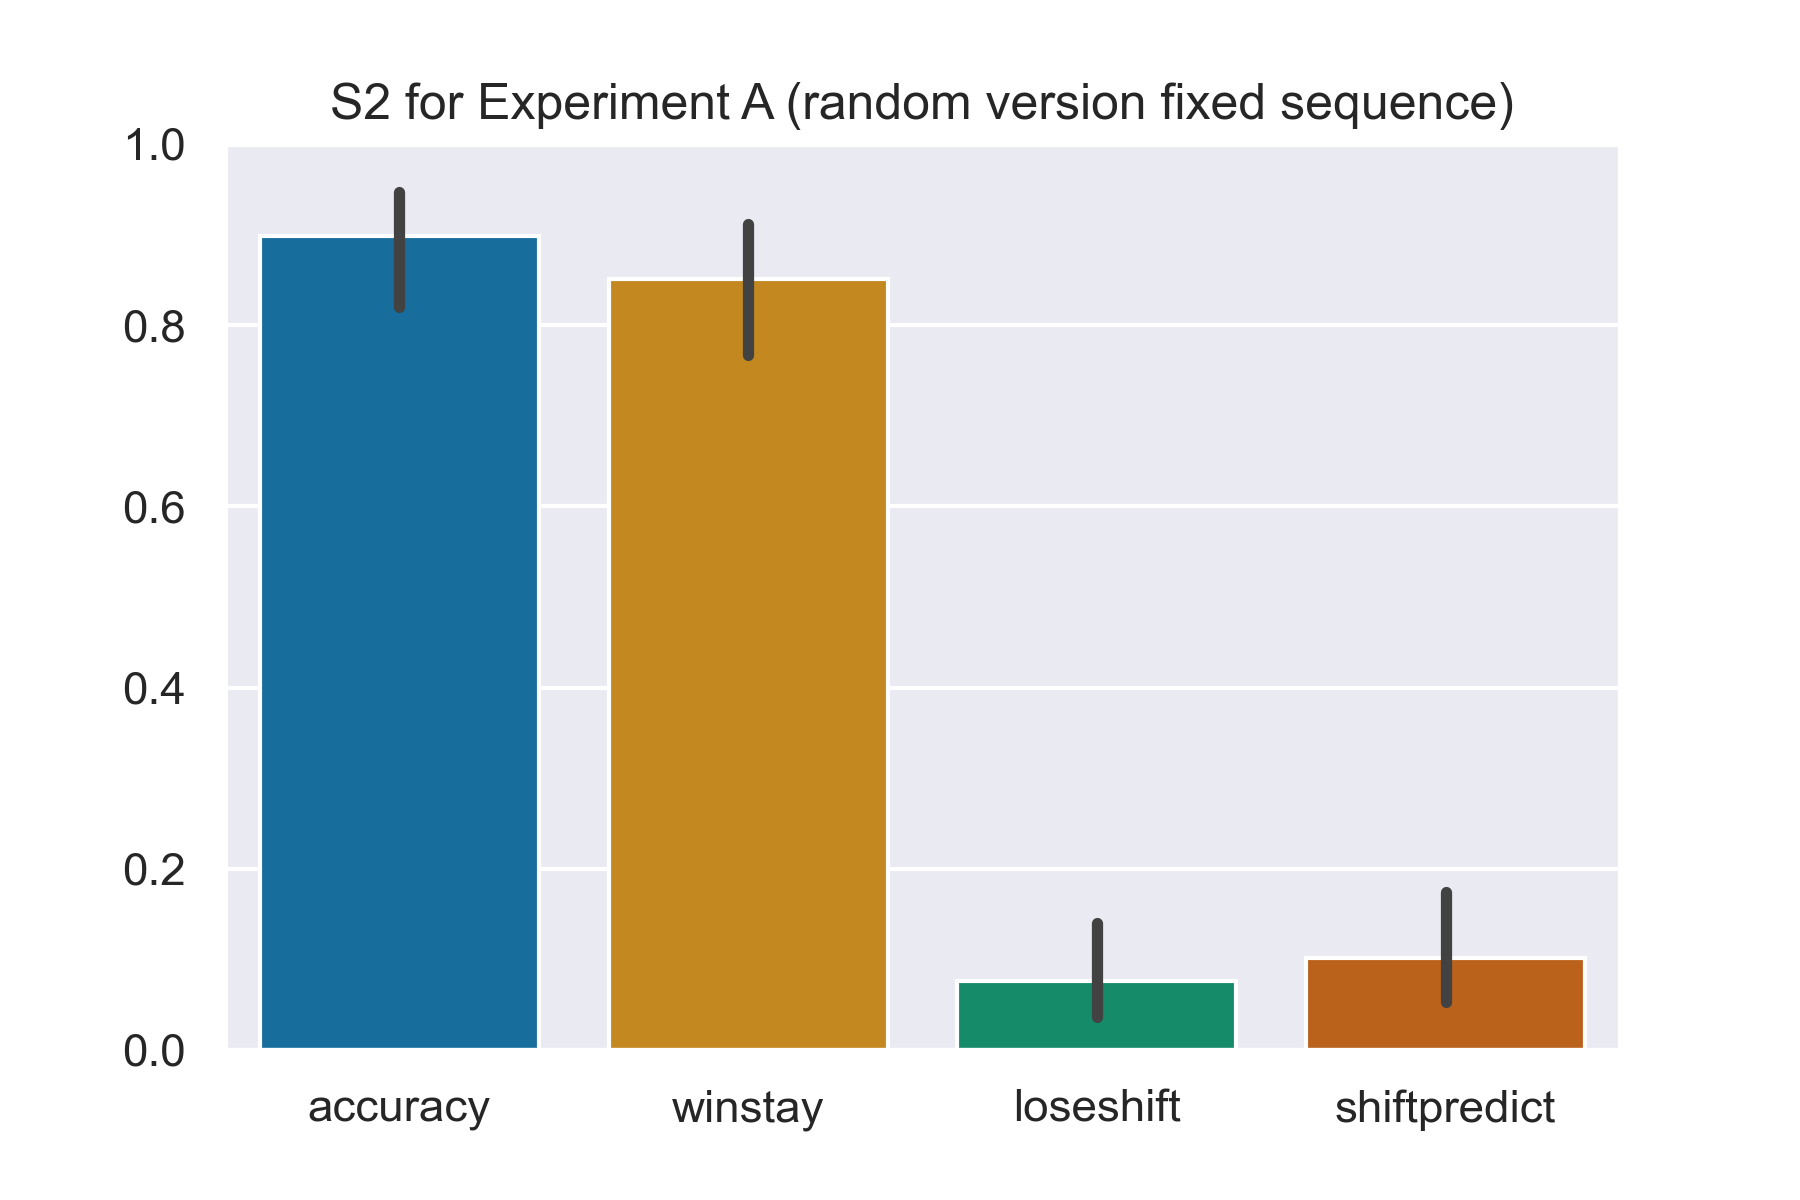
\includegraphics[width=0.9\linewidth, height=4cm]{plots/expA_s2.png}
\label{fig:expA2}
\end{subfigure}
\begin{subfigure}{0.33\textwidth}
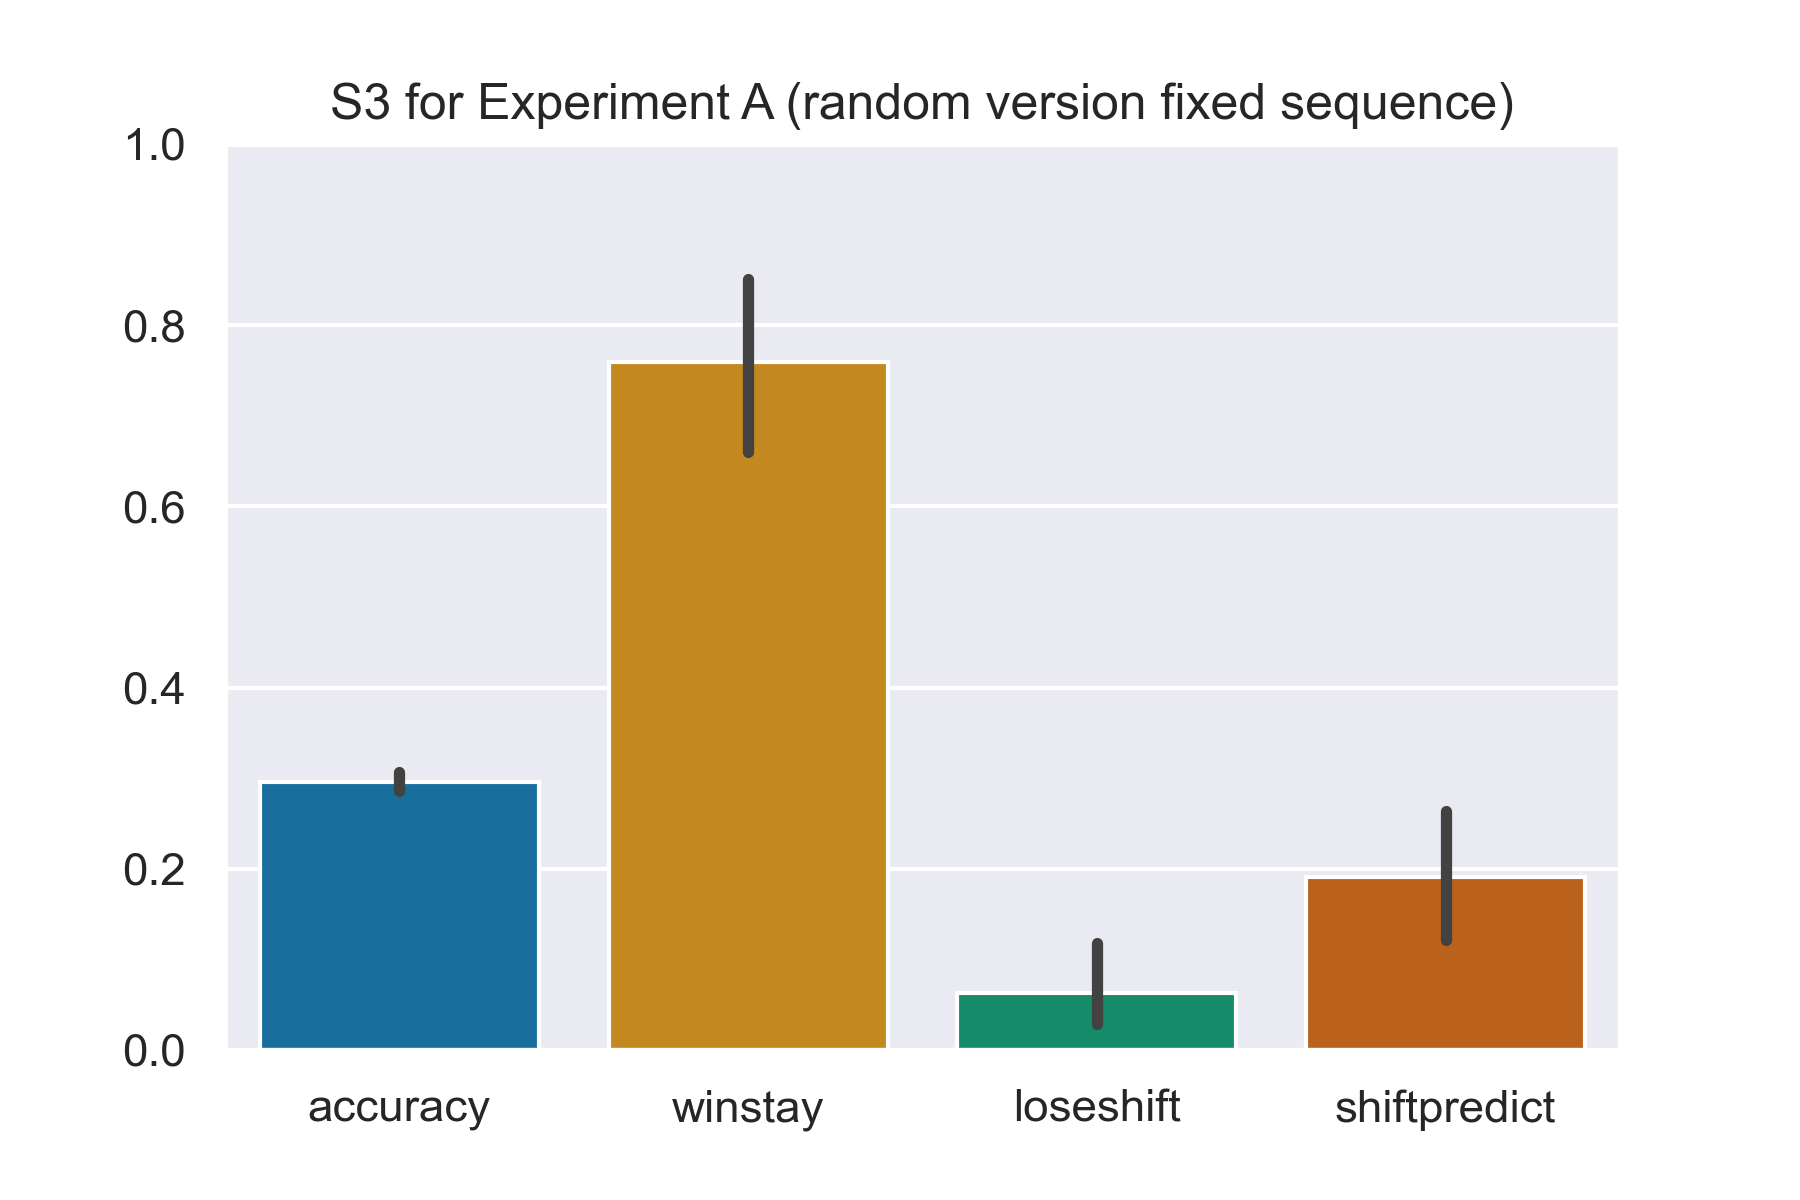
\includegraphics[width=0.9\linewidth, height=4cm]{plots/expA_s3.png}
\label{fig:expA3}
\end{subfigure}

\begin{subfigure}{0.33\textwidth}
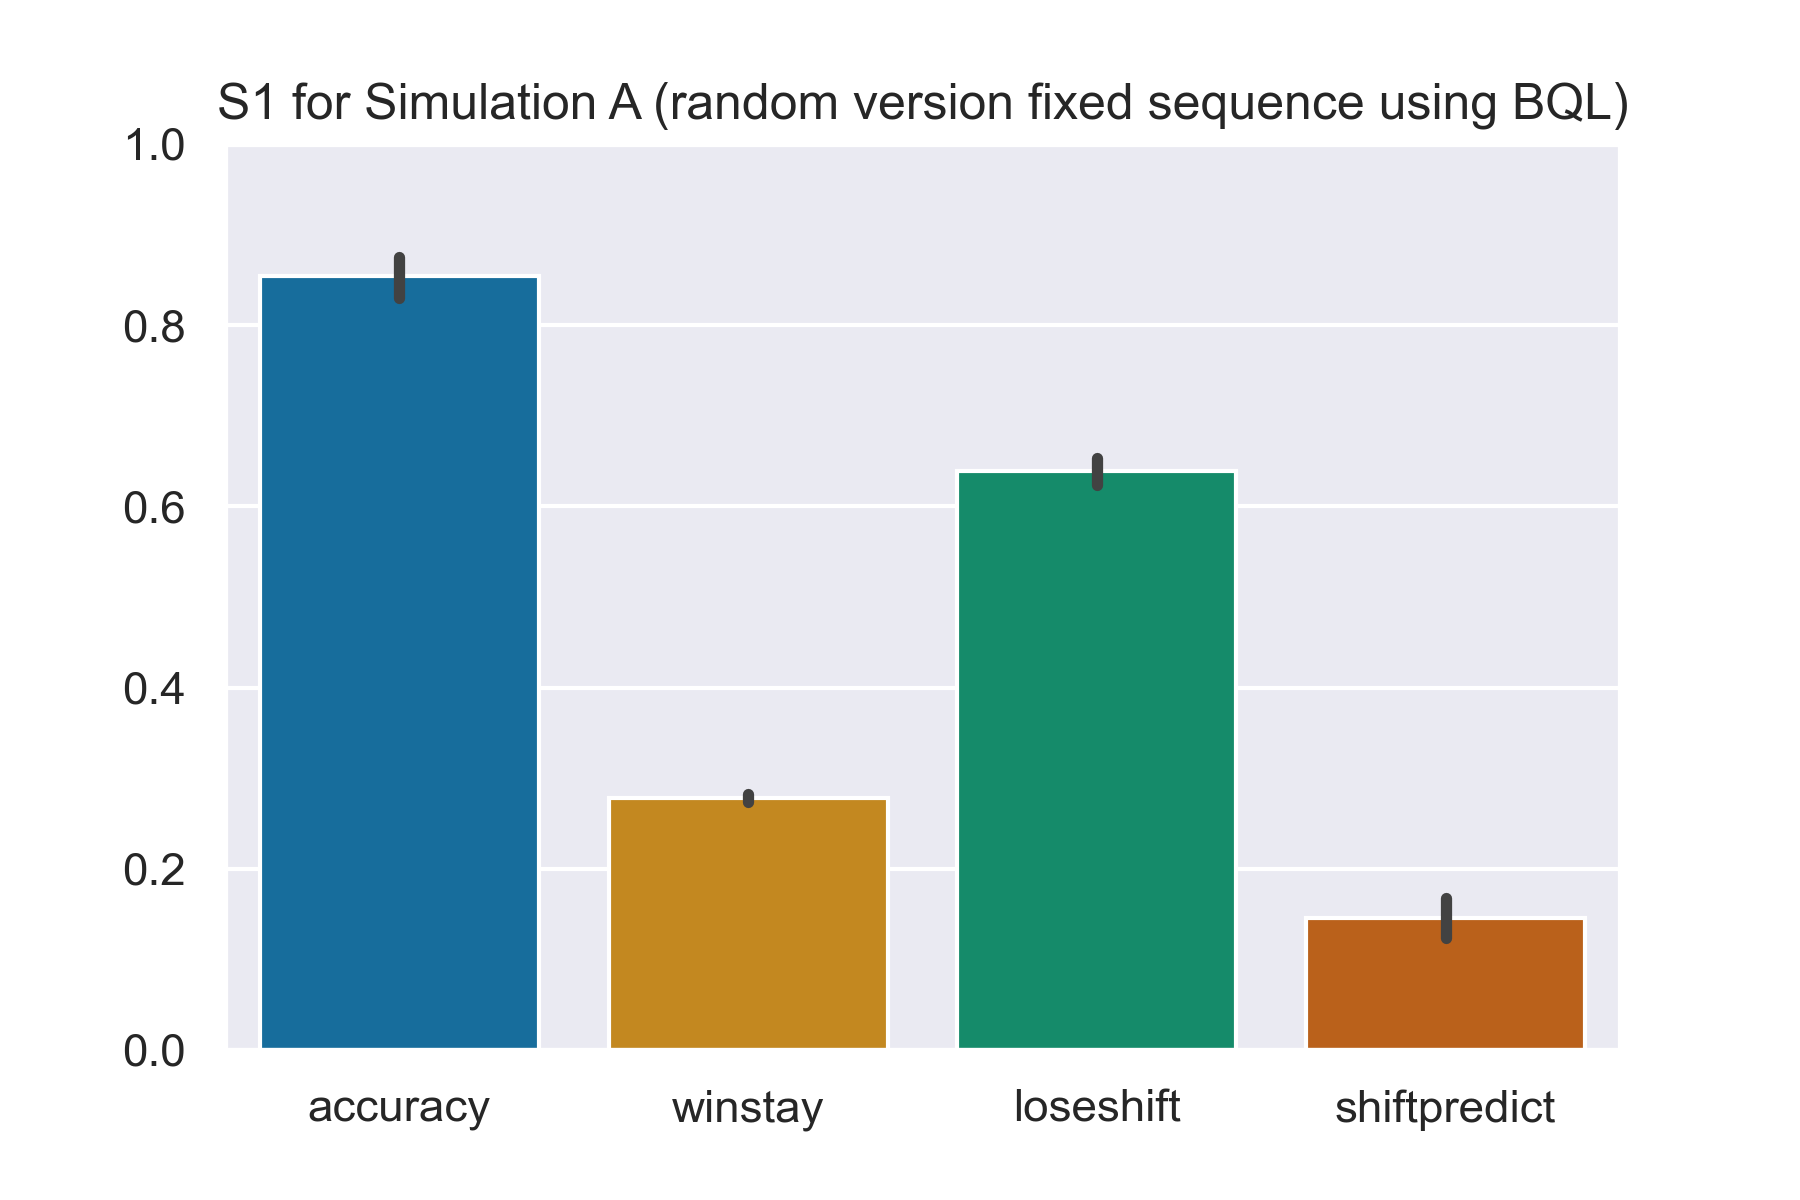
\includegraphics[width=0.9\linewidth, height=4cm]{plots/simA_s1.png} 
\label{fig:simA1}
\end{subfigure}
\begin{subfigure}{0.33\textwidth}
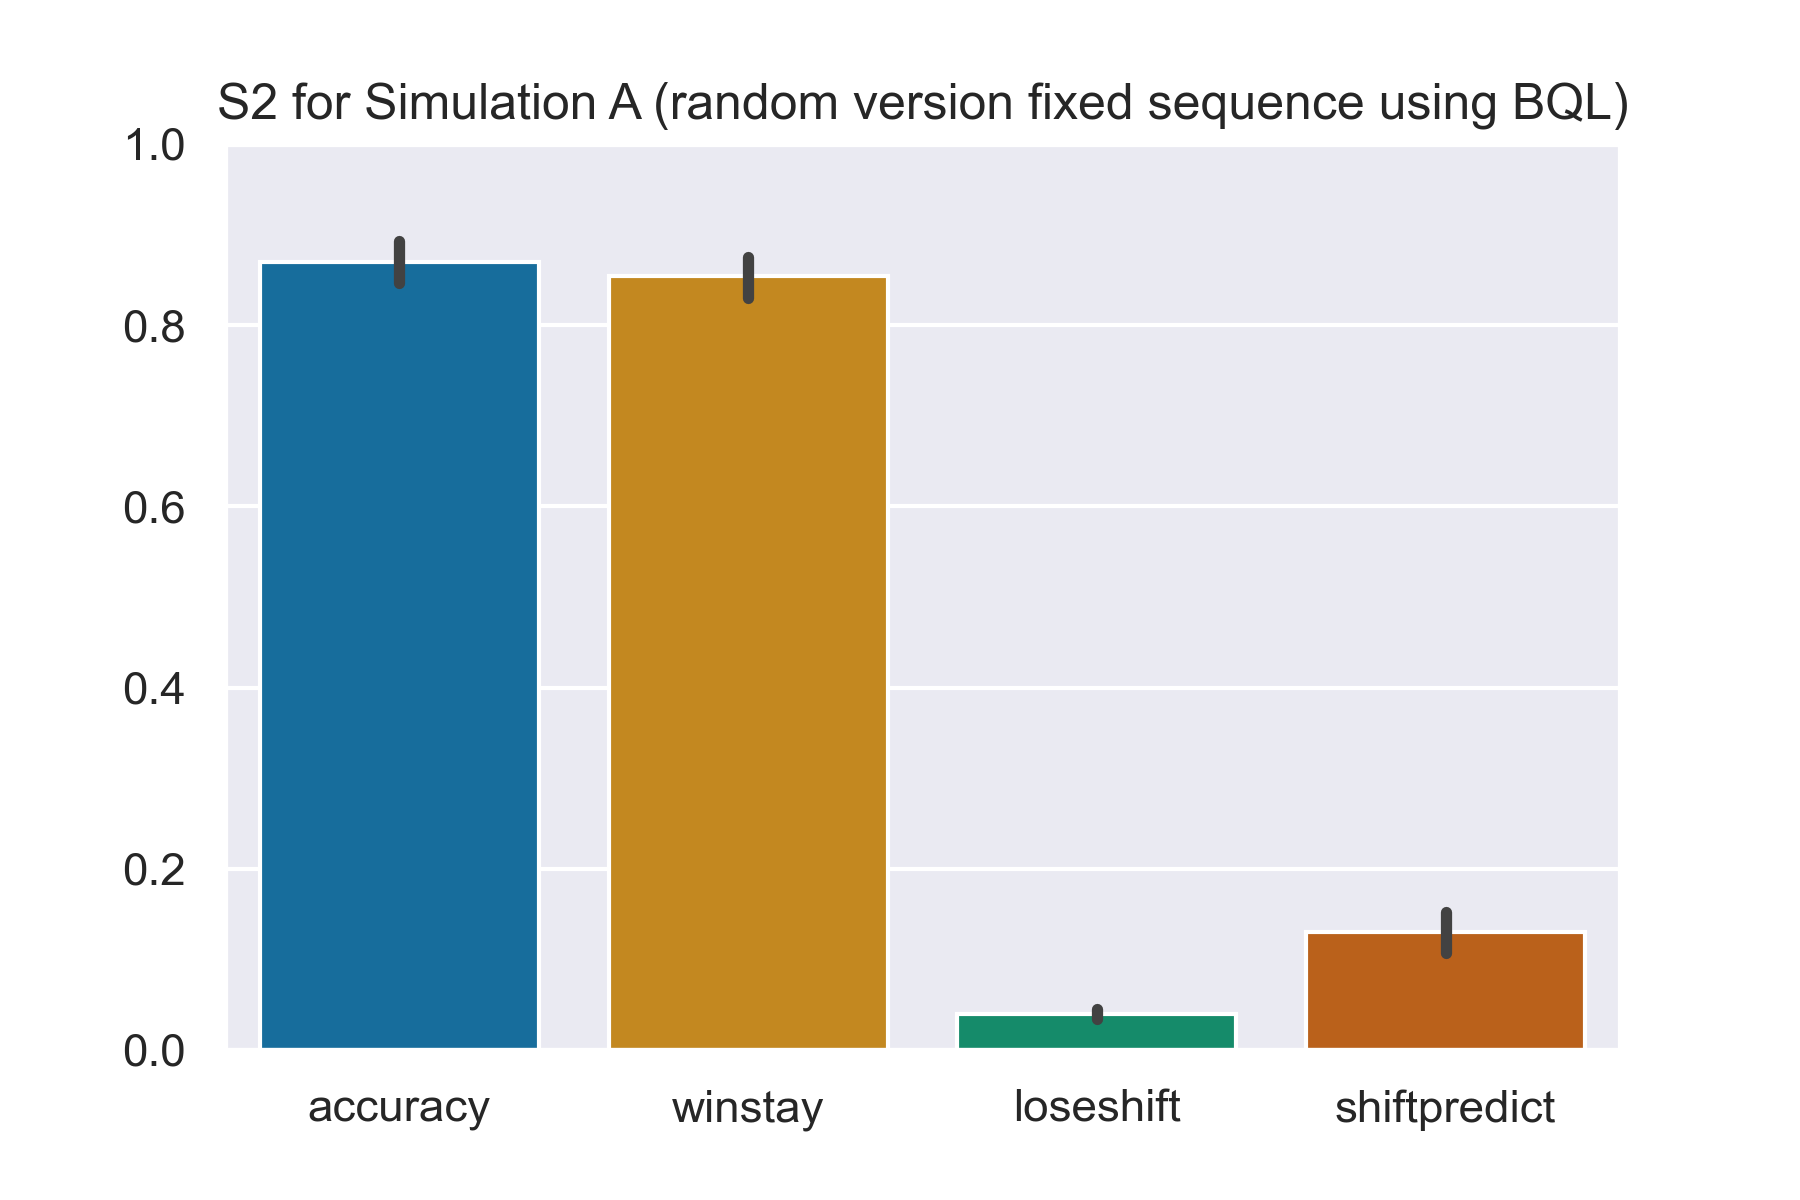
\includegraphics[width=0.9\linewidth, height=4cm]{plots/simA_s2.png}
\label{fig:simA2}
\end{subfigure}
\begin{subfigure}{0.33\textwidth}
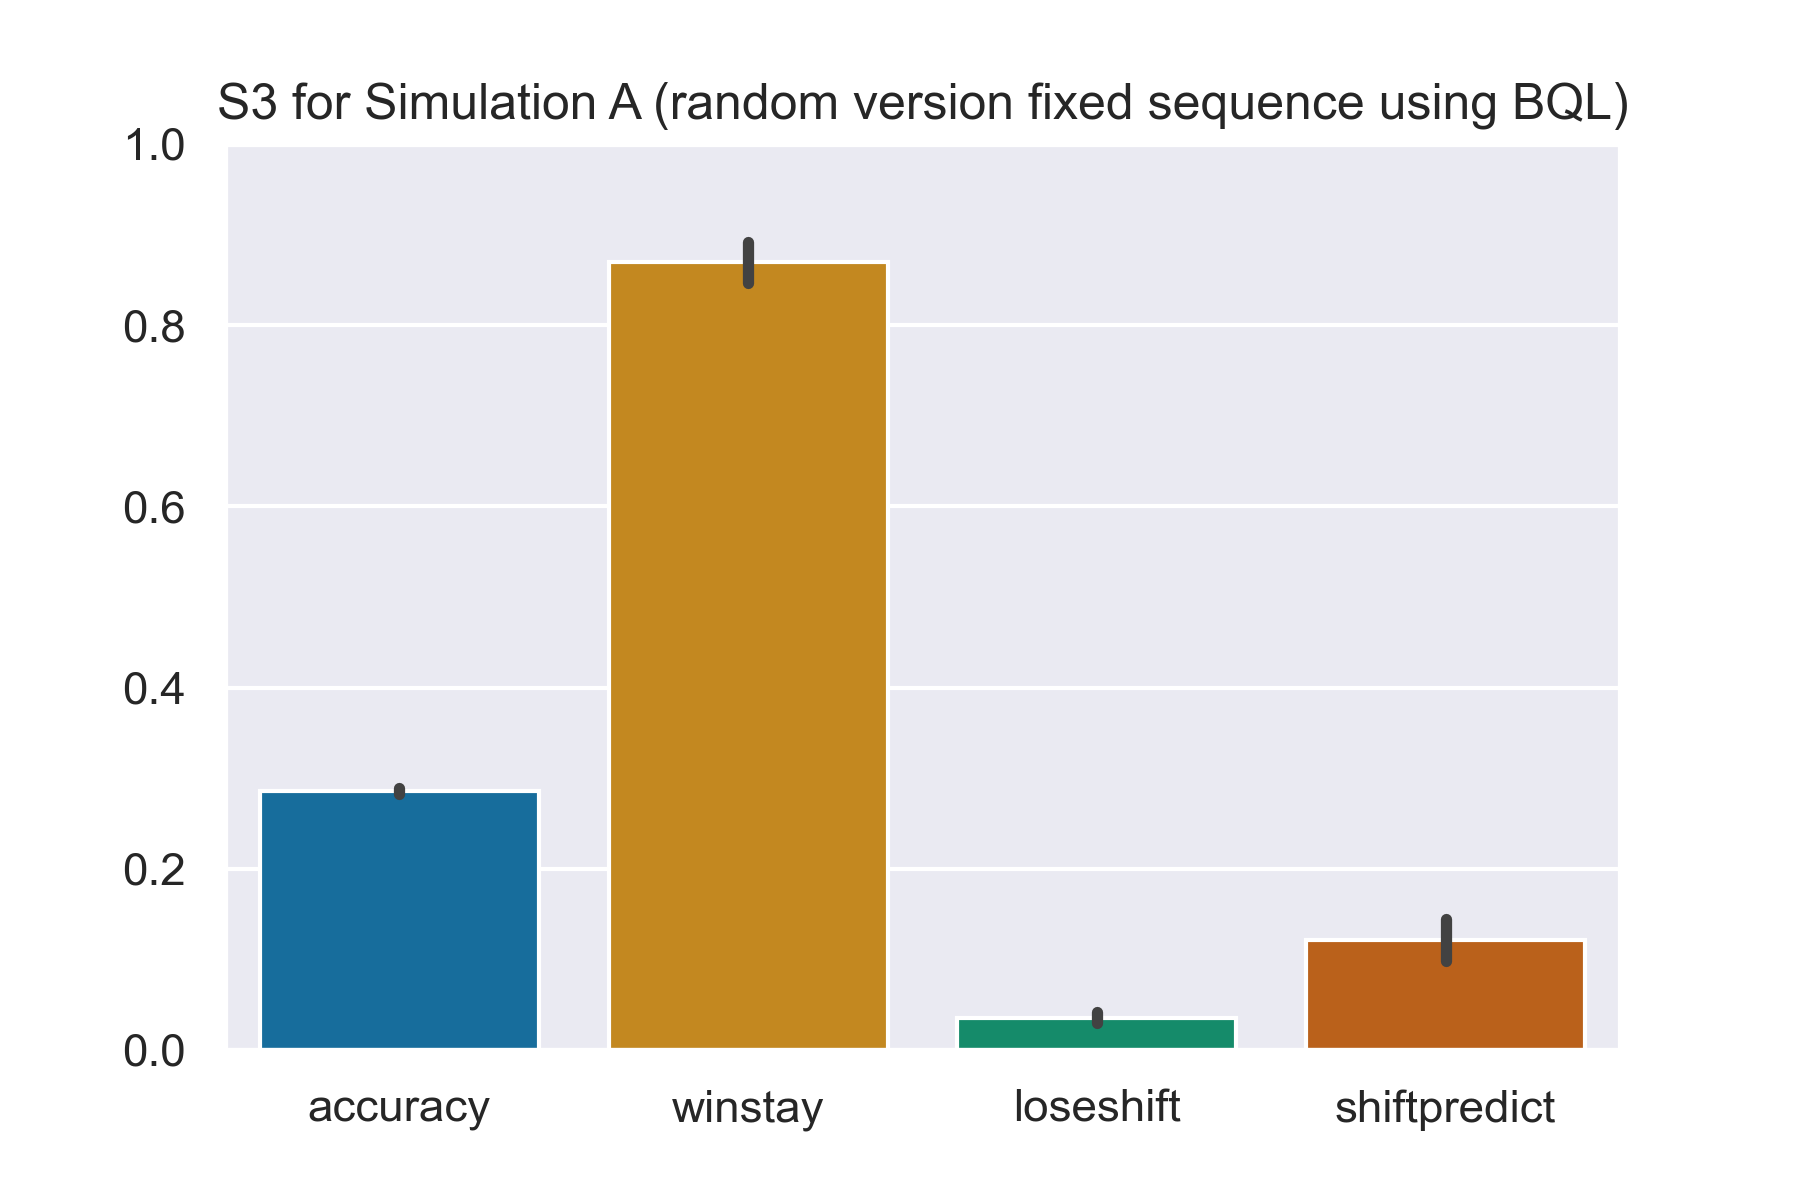
\includegraphics[width=0.9\linewidth, height=4cm]{plots/simA_s3.png}
\label{fig:simA3}
\end{subfigure}
 
\caption{Numbers on y axis represent probability and is averaged across participants. From left to right; S1, S2 and S3. Upper row: Experiment A (random version with fixed sequence for all participants). Lower Row: Simulation A (random bags with unique random sequence for each participant) using BQL}
\label{fig:figure2}
\end{figure*}

\subsection{Simulations}

Simulations of the task were based on Q-learning \cite{Watkins1992-rn}. Choices used softmax applied to the Q-values of the three actions (predict shape A, B or C on the next trial). The QL algorithm was adapted to calculate the prediction error as the difference between the next shape and the prediction of the next shape, i.e. the choice made on the current trial. This means we had three parameter values; learning rate alpha $(0 < \alpha < 1)$, temperature beta $(0 < \beta < 5)$ and discount parameter gamma $(0 < \gamma < 1)$. For each task, simulations used a total of 250 parameter combinations, and were run 100 times for each parameter combination. The simulation runs were then checked if they fulfilled the relaxed criteria of ‘solving’ the task which were that average accuracy on the first and second shape of each bag should be more than 50\% while the ‘shift prediction’ on the third shape of each bag should be more than 50\%. We also scored each trial with win-stay, lose-shift as for the human participants.

\subsubsection{State codings} In the ‘basic’ QL model (BQL), we simply coded each shape as a binary array of length three, where circle was [1, 0, 0], triangle [0, 1, 0] and square [0, 0, 1]. For the state enhanced QL model (SEQL) we used the same coding for the shapes but added three bits for position, so for example the first circle in a bag was [1, 0, 0, 1, 0, 0], the second circle [1, 0, 0, 0, 1, 0] and the third circle [1, 0, 0, 0, 0, 1].

\section{Results}

We define S1 as the first occurrence in a set of 3 repeats of the same shape; S2 is the second repeat of the shape, and S3 the third. In other words, S1 is the first shape in a bag, S2 the second and S3 the third. All scores are averaged across participants unless otherwise specified.

\subsubsection{Experiment A: random bags with fixed sequence for all participants}
Participants had high accuracy on S1 and S2 (Figure 2, upper row), with an average accuracy of .89 (SD .17) for S1, .90 (SD .17) for S2 and .30 (SD .03) for S3. Shift prediction had an average of .11 (SD .17) on S1, .10 (SD .17) on S2 and .19 (SD .19) for S3. For shift prediction, there was a significant difference between S3 and S2 (paired t-test; $t(26)=2.75, p=0.01$) as well as S3 and S1 (paired t-test; $t(26)=2.30, p=0.03$). Meanwhile, lose-shift was high on S1 (mean .66, SD .06) and win-stay high on S2 (.85, SD .20) and S3 (.76, SD .25), as can be seen in Figure 2. This shows participants did not learn the underlying pattern and instead adopted a win-stay, lose-shift behaviour quite quickly and stayed with that throughout the task (see code repository).

\subsubsection{Simulation A: random bags with fixed sequence (BQL)}

Many parameter combinations could show qualitatively similar behaviour as the human subjects in Experiment A. The one shown in Figure 2 uses $\alpha = 0.41, \beta = 0.01, \gamma = 0.61$ for 270 trials. Our QL model takes slightly longer to learn (but still within 99 trials, to compare with experiments B-D, see code repository) and similar shift prediction for S1 (.15, SD .12), S2 (.13, SD .12) and S3 (.12, SD .12) as the human participants. It is worth noting that the slightly higher shift prediction on S3 in experiment A is not reproduced here.

% expB and simB1 and simB2 results

\begin{figure*}[t]
\centering
\captionsetup{justification=centering}

\begin{subfigure}{0.33\textwidth}
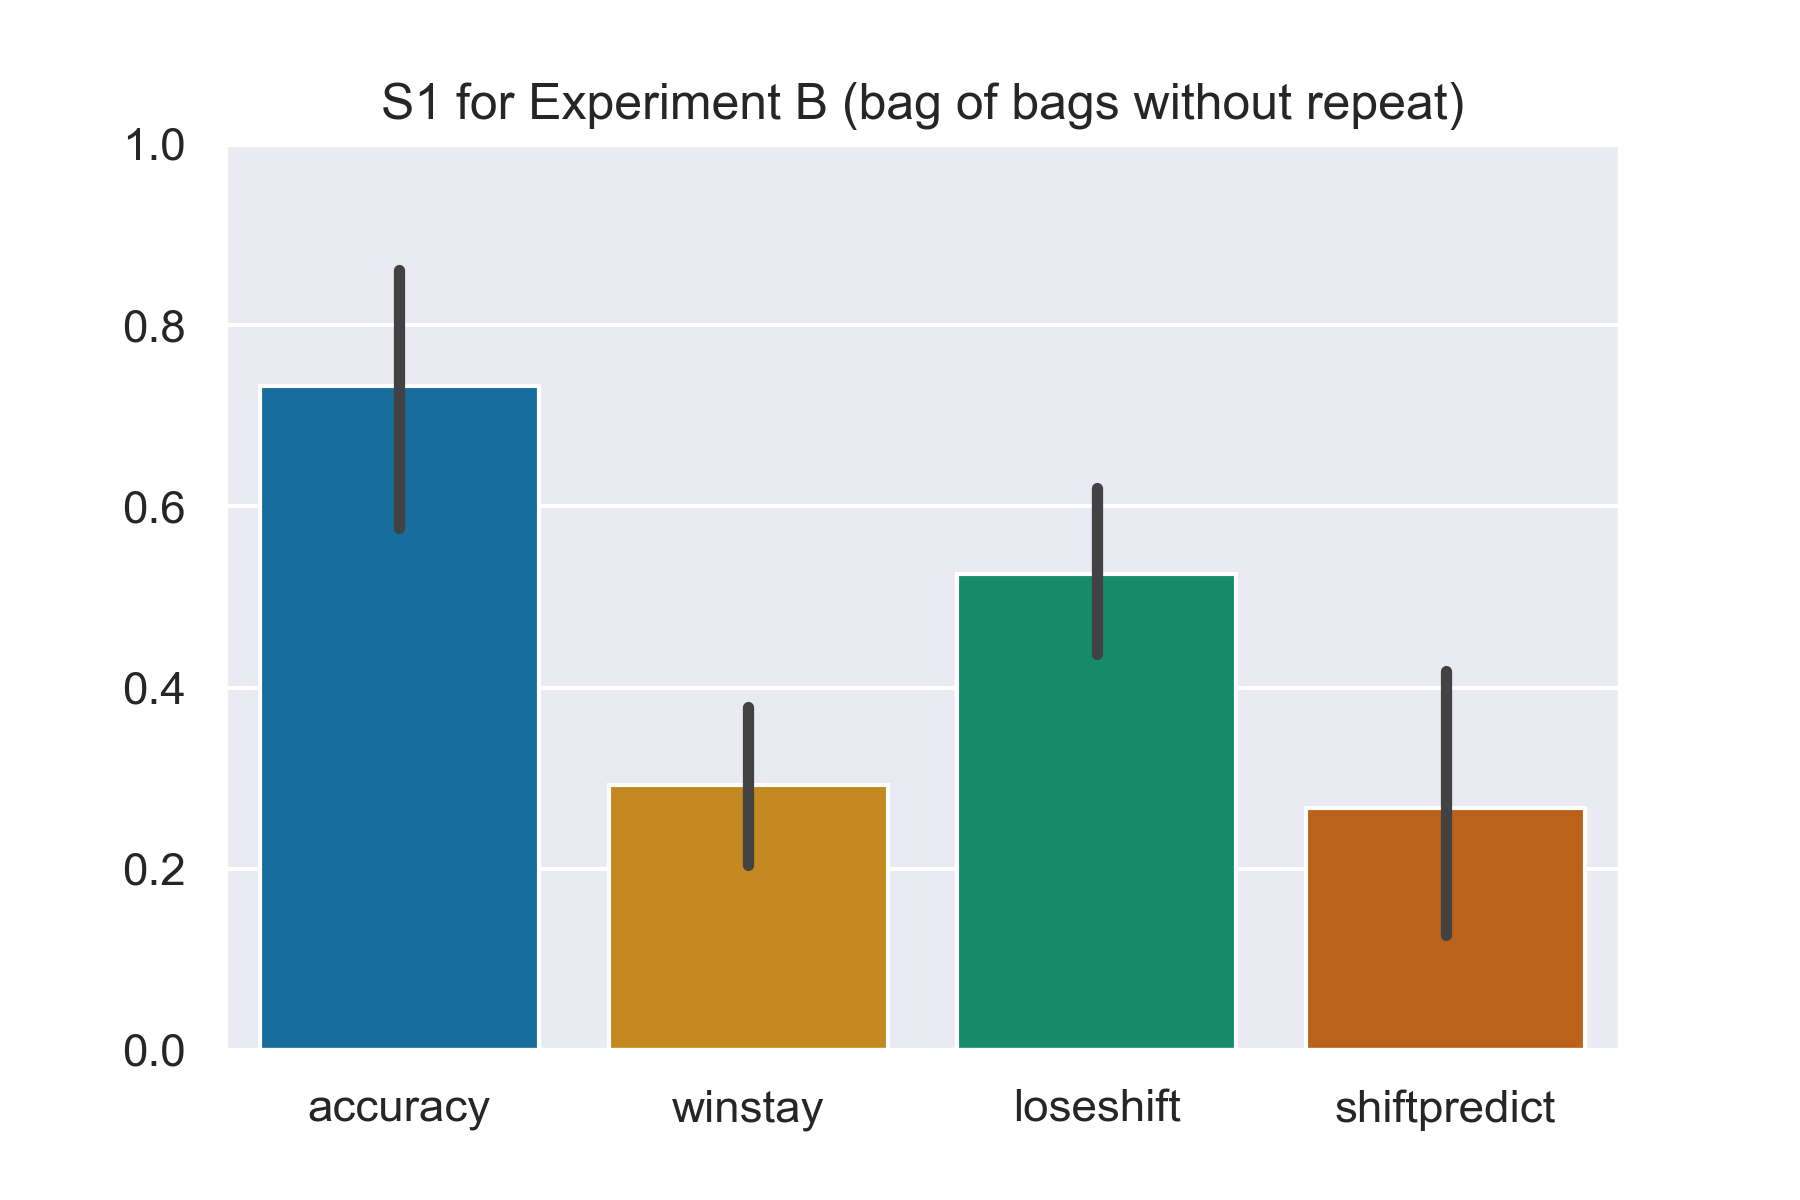
\includegraphics[width=0.9\linewidth, height=4cm]{plots/expB_s1.png} 
\label{fig:expB1}
\end{subfigure}
\begin{subfigure}{0.33\textwidth}
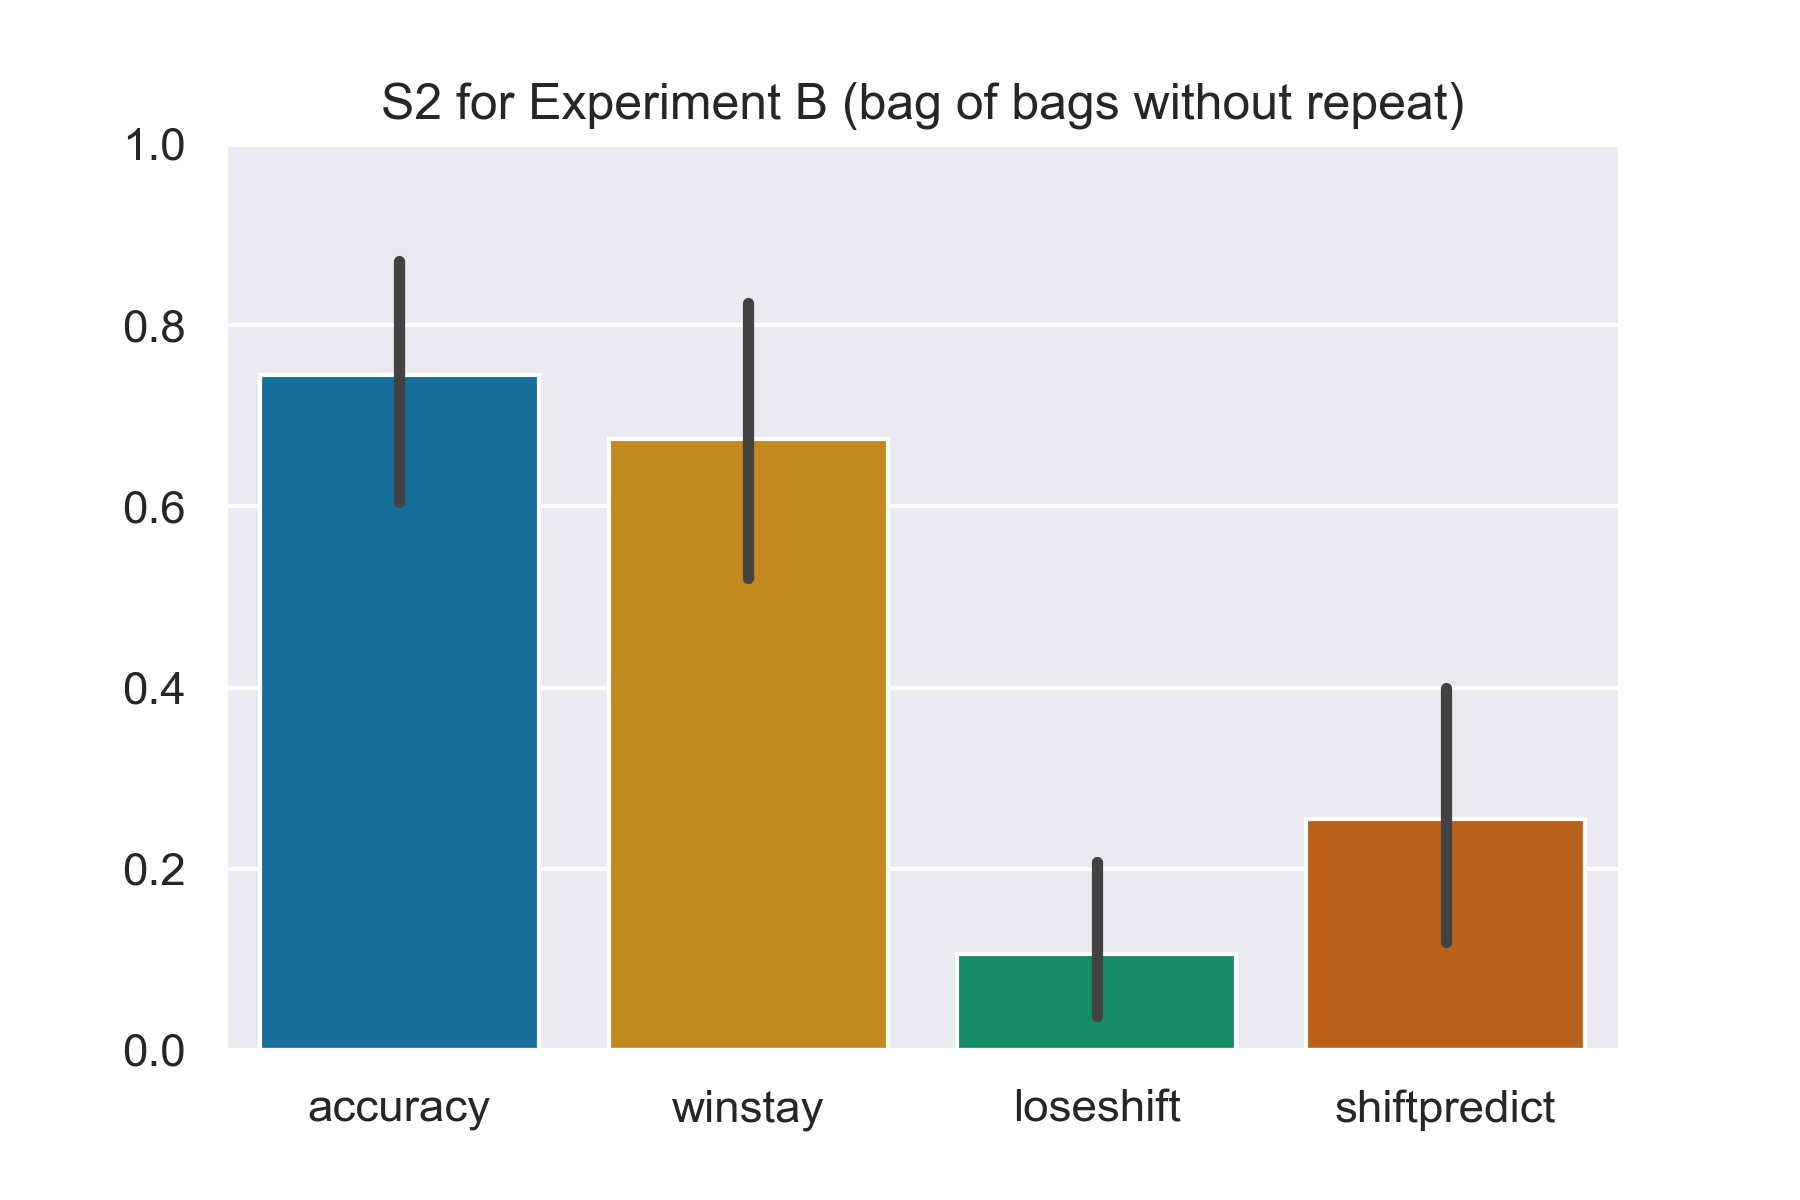
\includegraphics[width=0.9\linewidth, height=4cm]{plots/expB_s2.png}
\label{fig:expB2}
\end{subfigure}
\begin{subfigure}{0.33\textwidth}
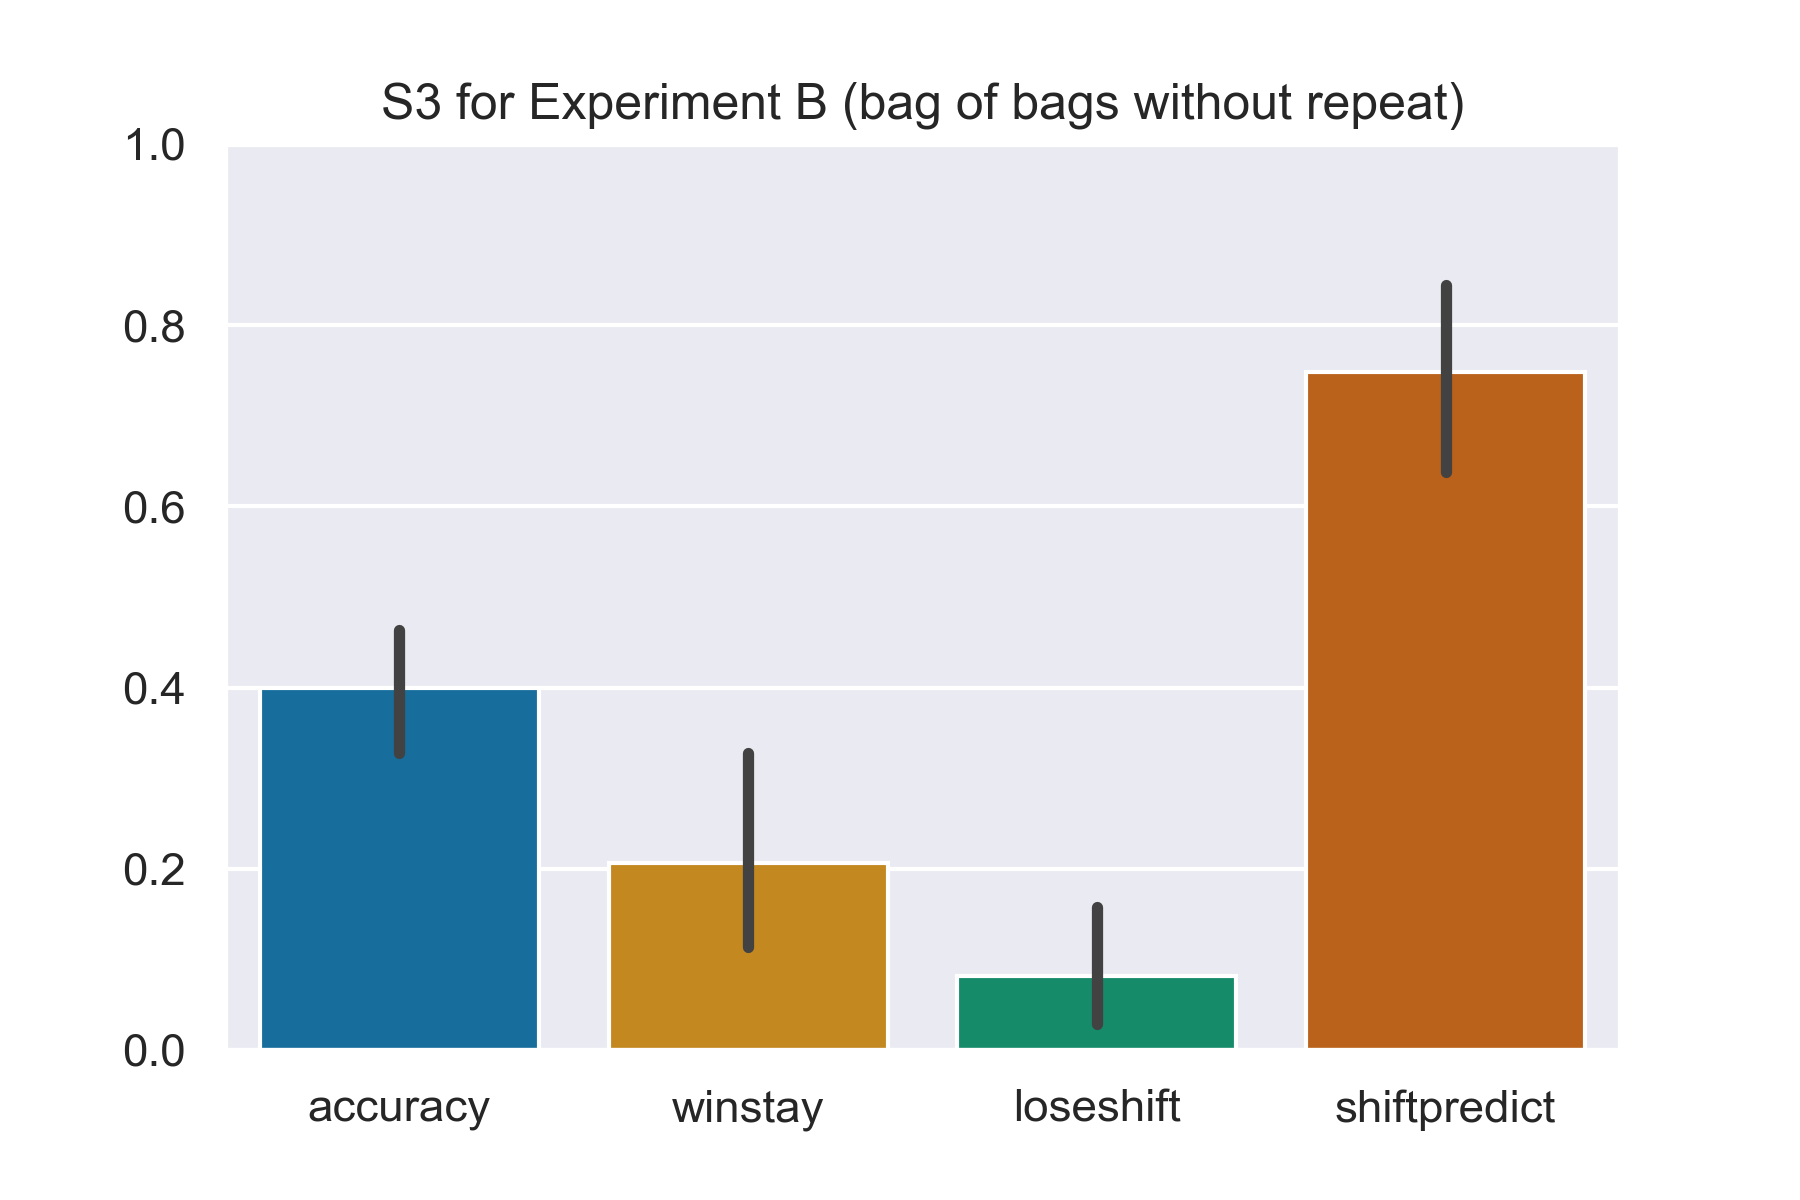
\includegraphics[width=0.9\linewidth, height=4cm]{plots/expB_s3.png}
\label{fig:expB3}
\end{subfigure}

\begin{subfigure}{0.33\textwidth}
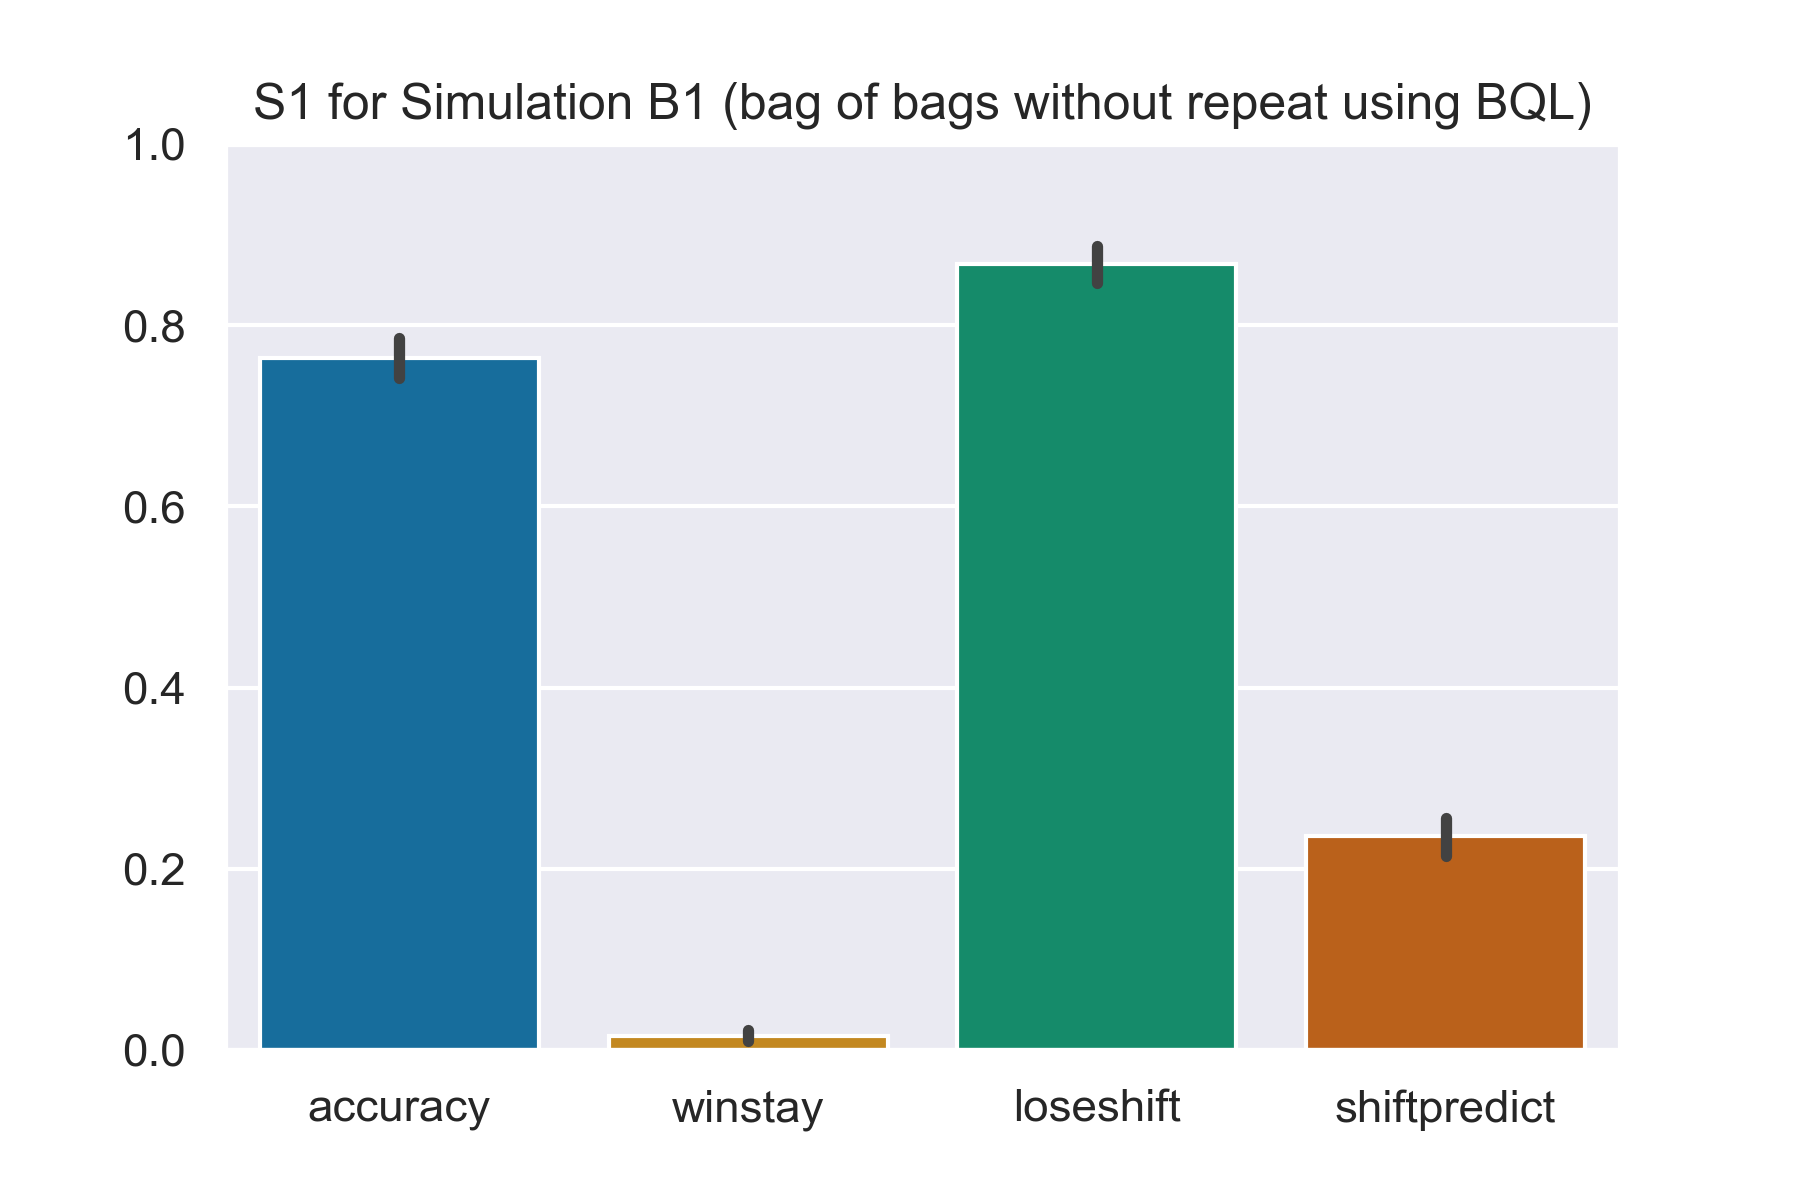
\includegraphics[width=0.9\linewidth, height=4cm]{plots/simB1_s1.png} 
\label{fig:simB11}
\end{subfigure}
\begin{subfigure}{0.33\textwidth}
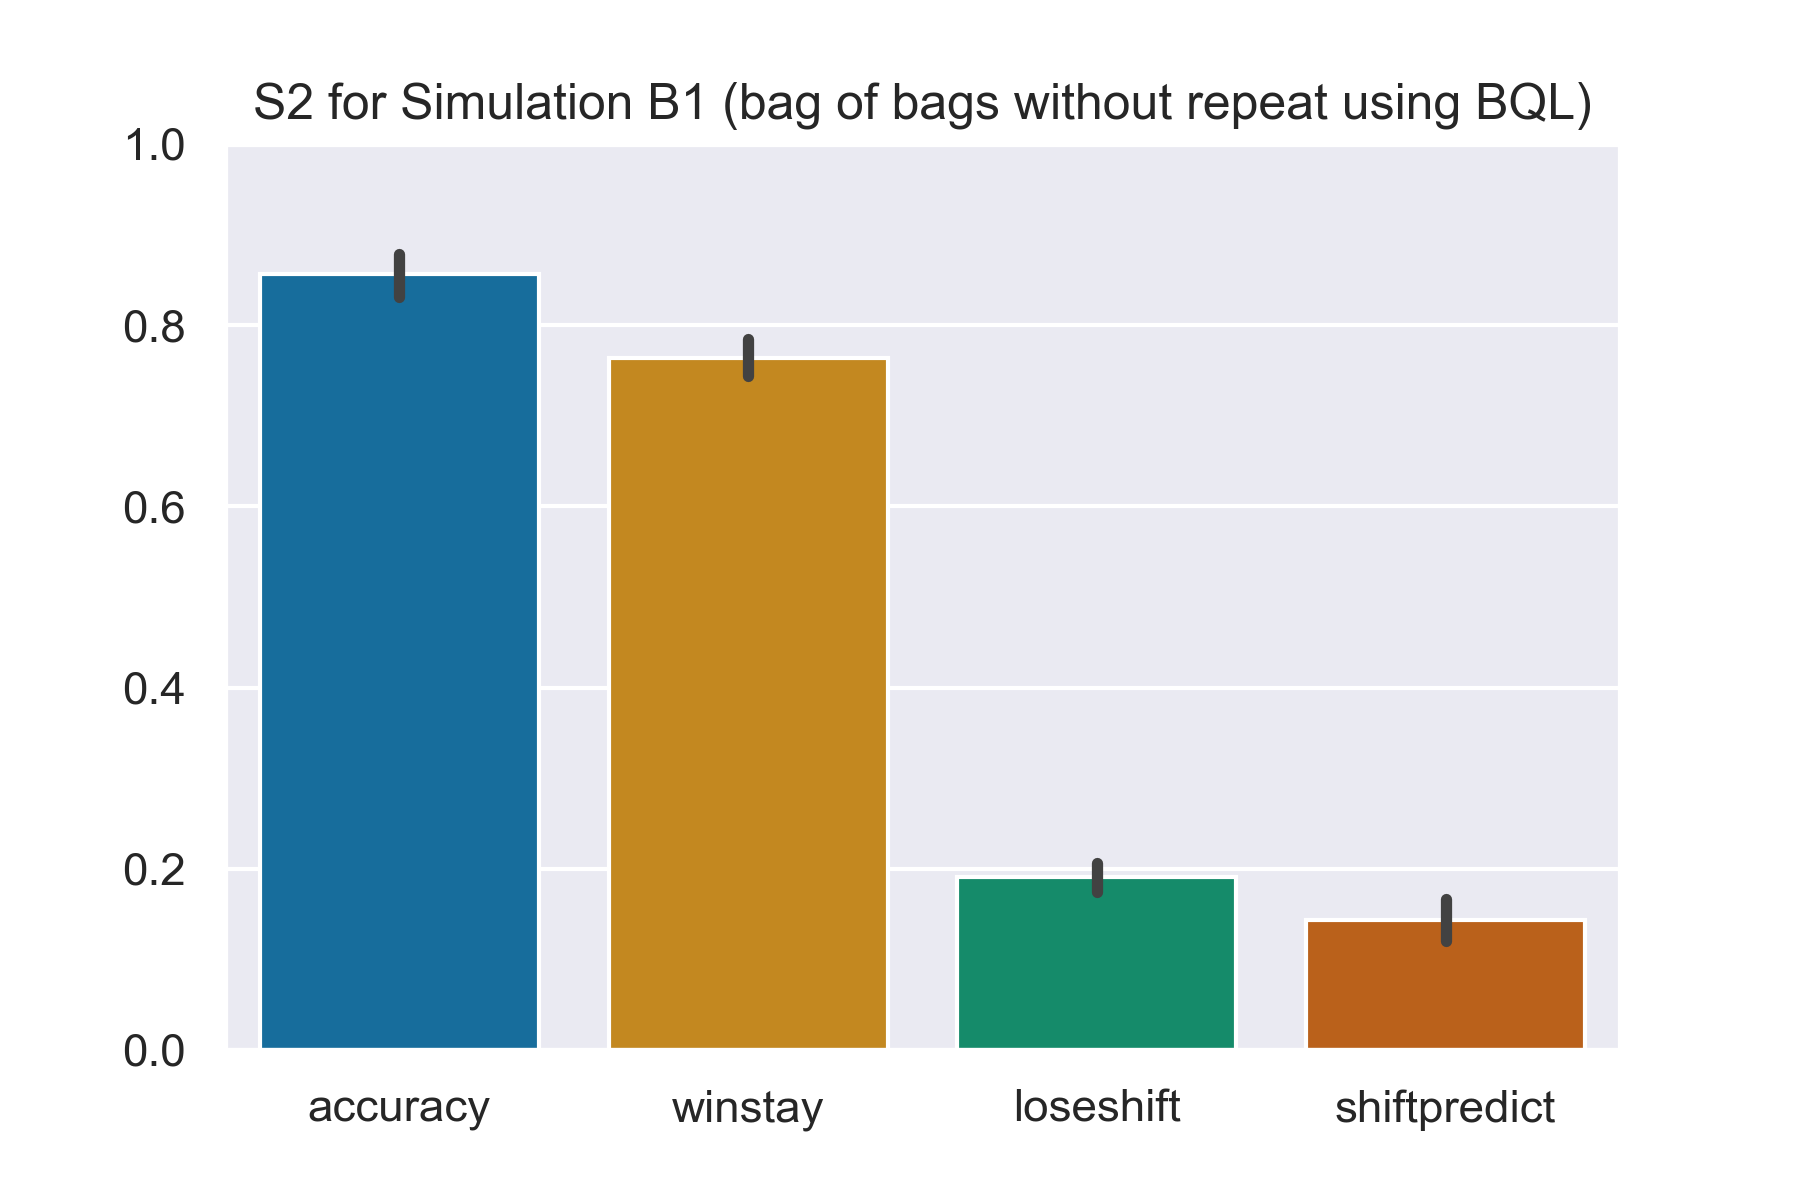
\includegraphics[width=0.9\linewidth, height=4cm]{plots/simB1_s2.png}
\label{fig:simB12}
\end{subfigure}
\begin{subfigure}{0.33\textwidth}
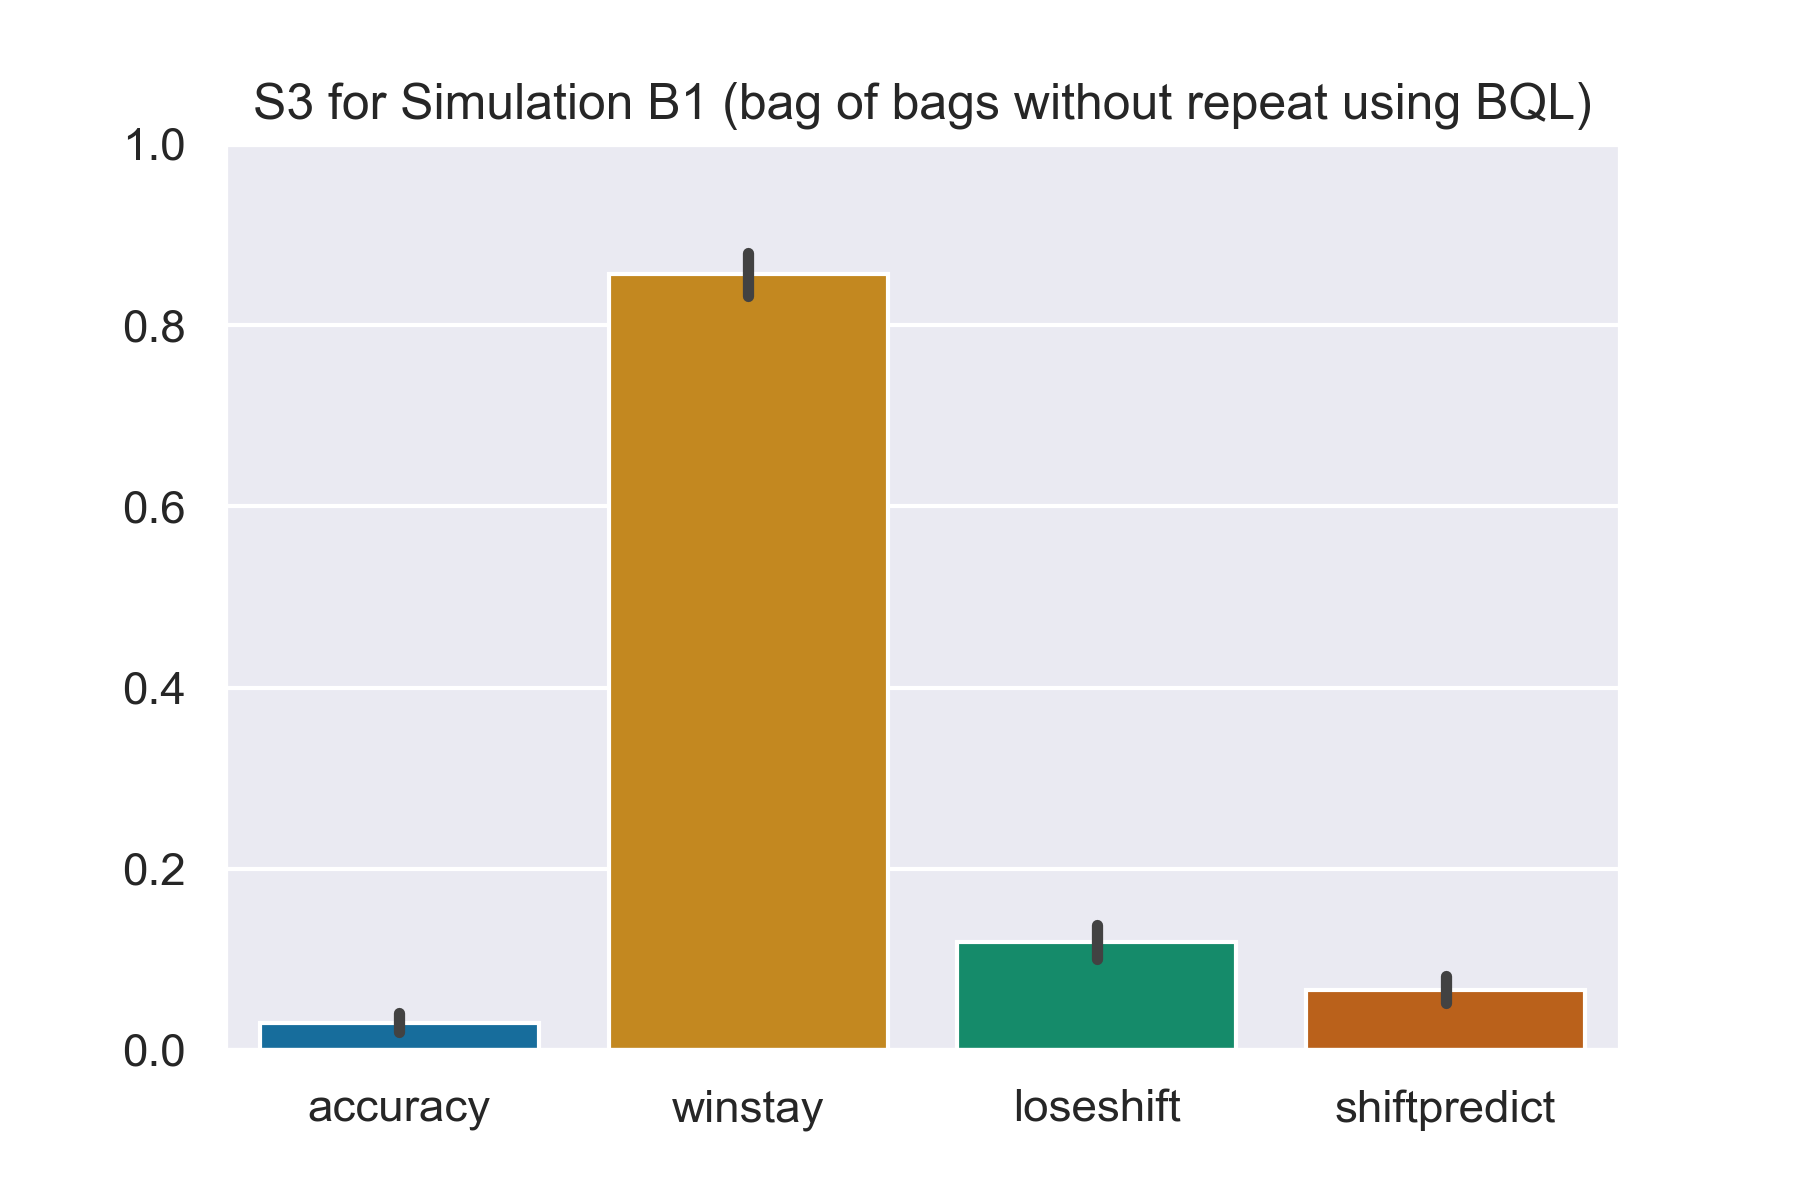
\includegraphics[width=0.9\linewidth, height=4cm]{plots/simB1_s3.png}
\label{fig:simB13}
\end{subfigure}

\begin{subfigure}{0.33\textwidth}
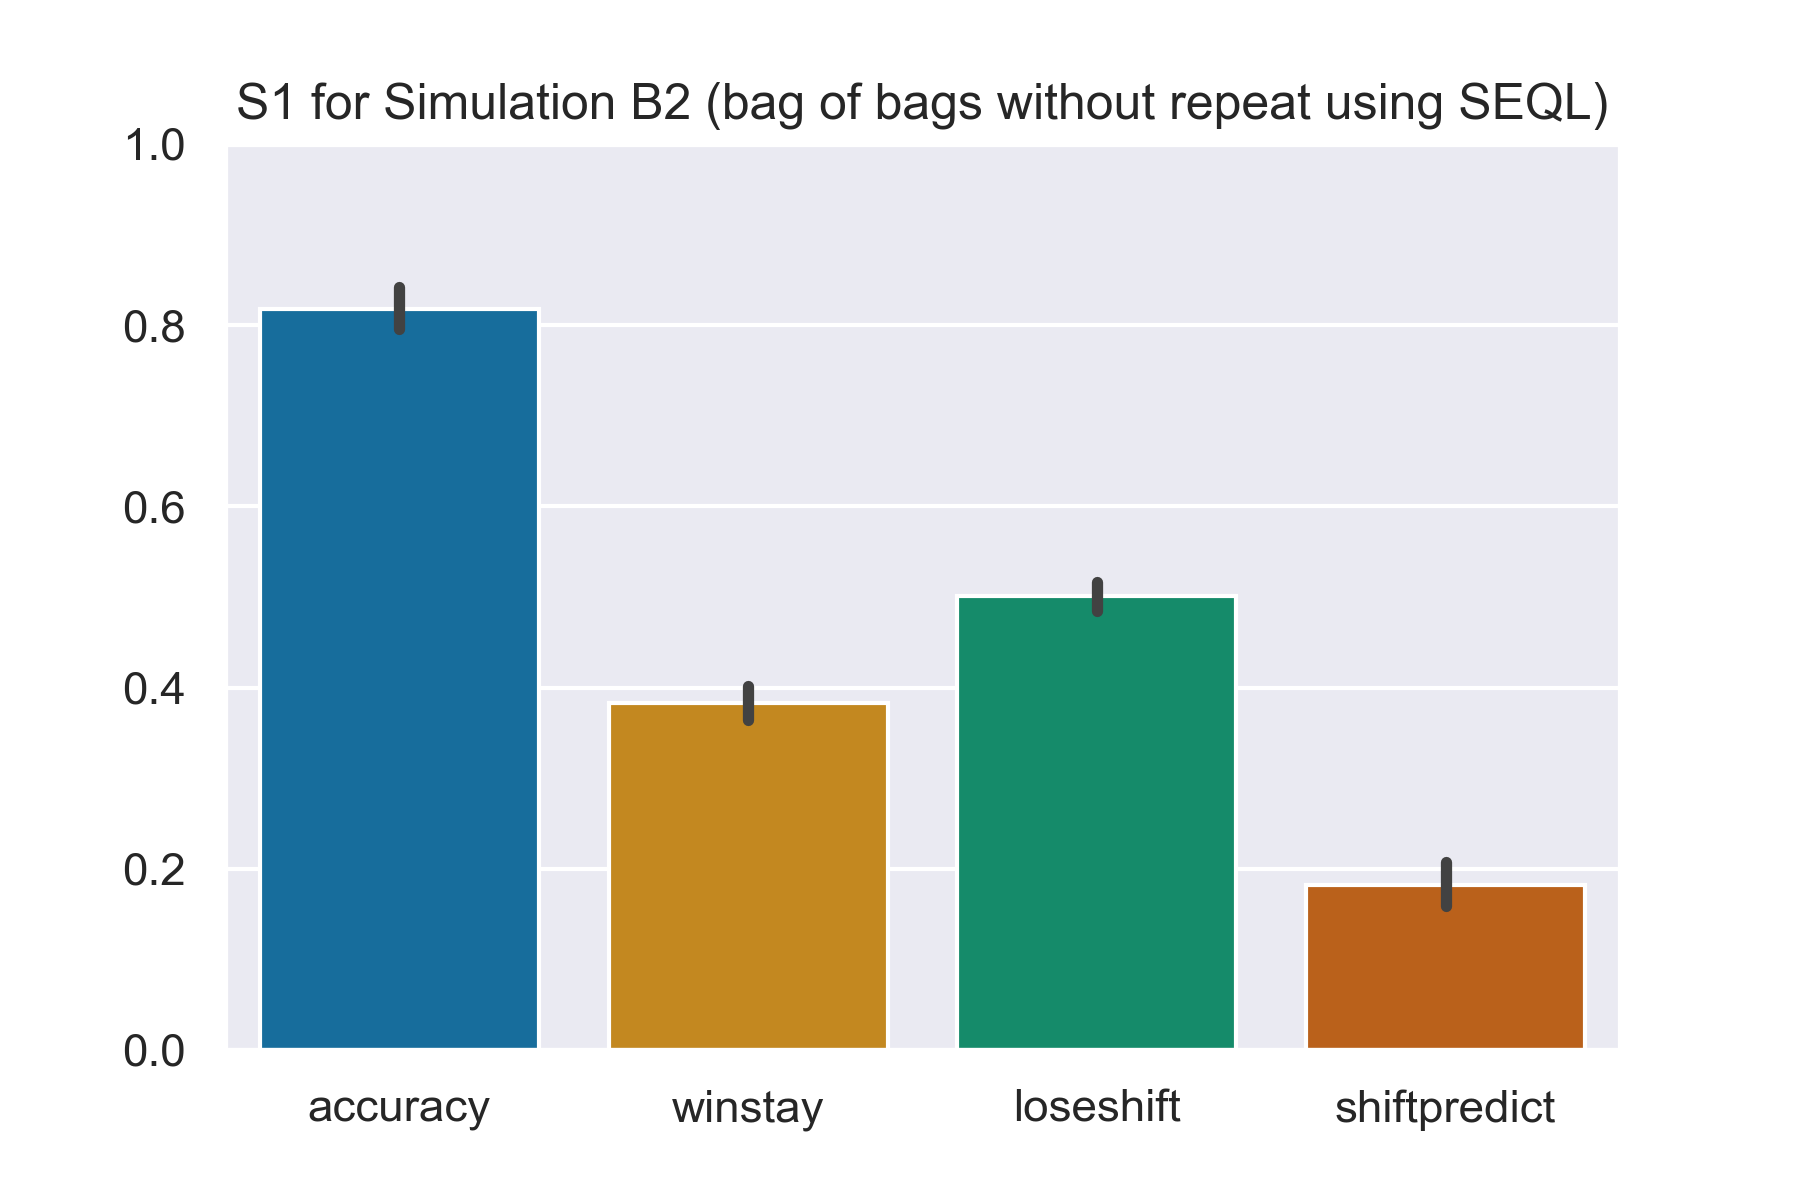
\includegraphics[width=0.9\linewidth, height=4cm]{plots/simB2_s1.png} 
\label{fig:simB21}
\end{subfigure}
\begin{subfigure}{0.33\textwidth}
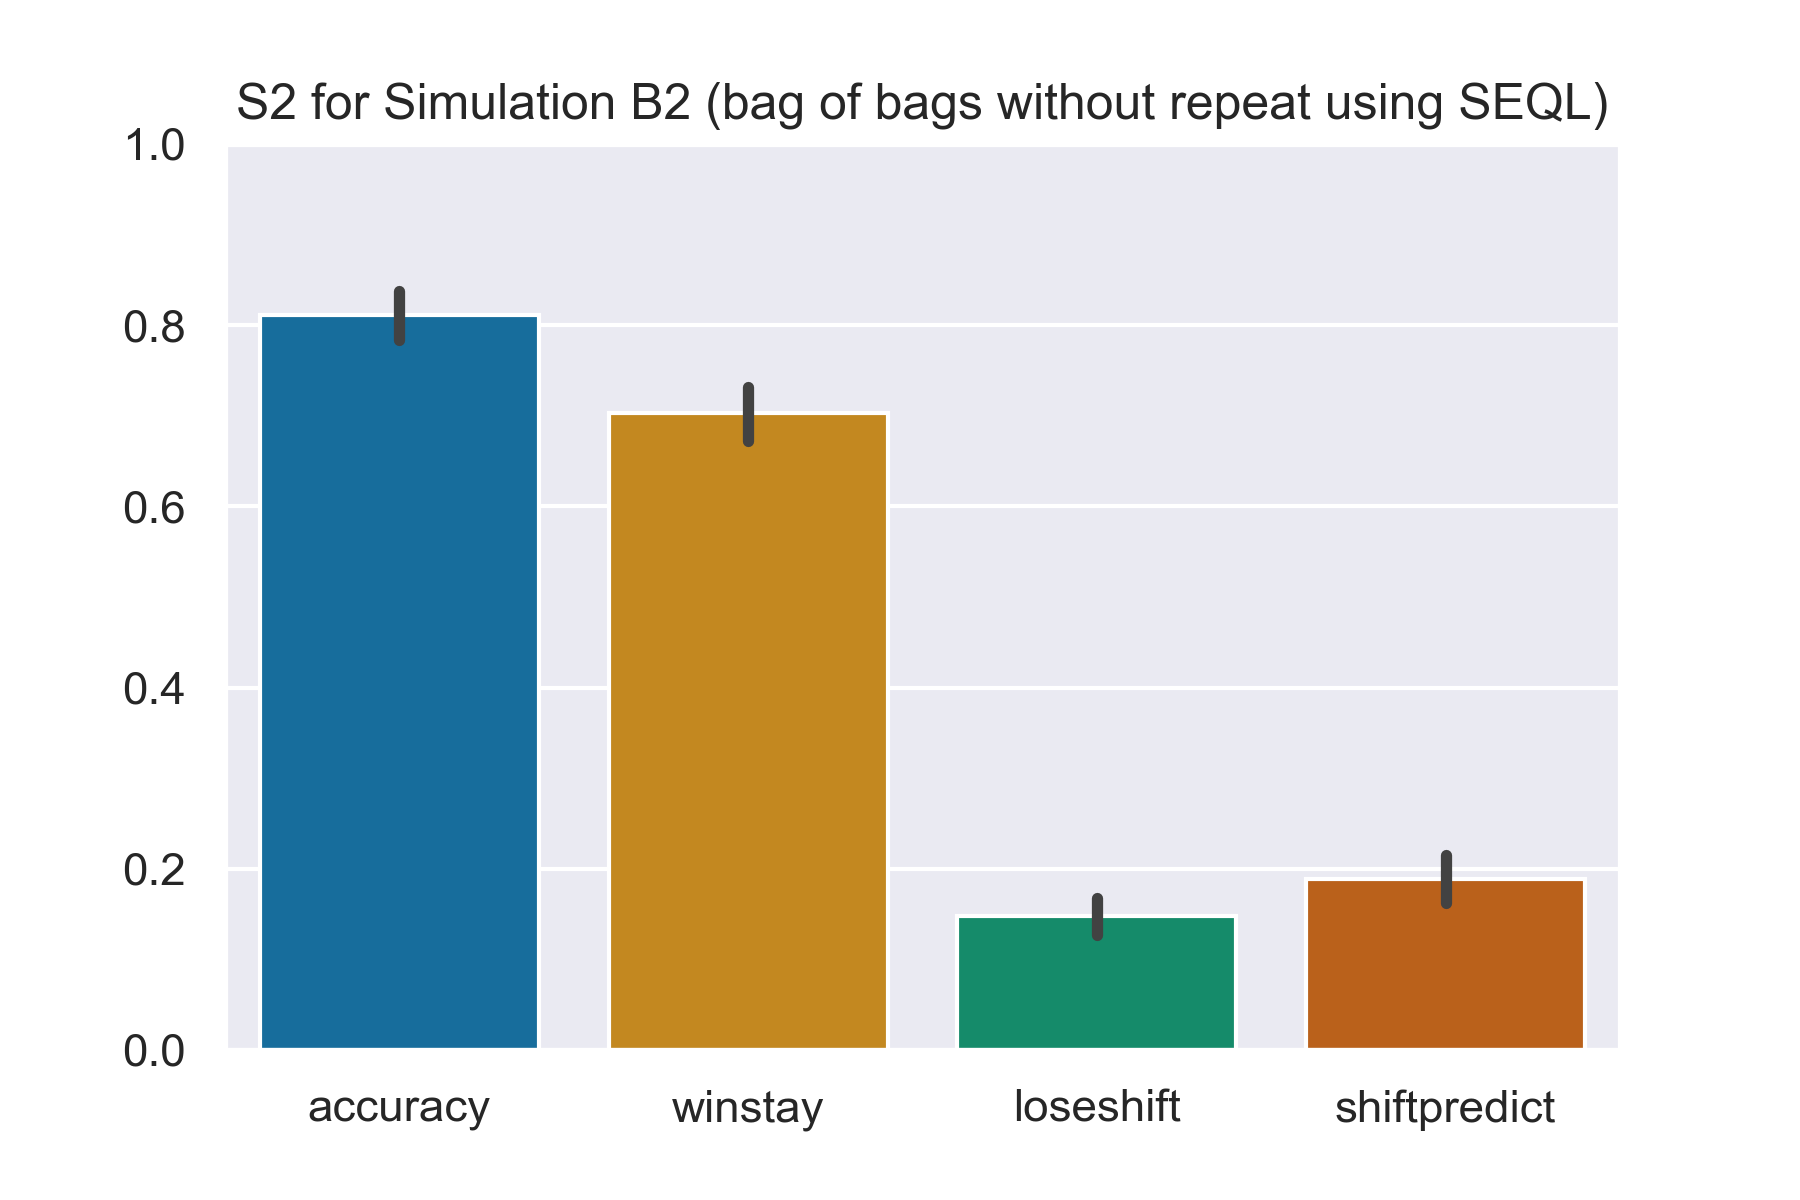
\includegraphics[width=0.9\linewidth, height=4cm]{plots/simB2_s2.png}
\label{fig:simB22}
\end{subfigure}
\begin{subfigure}{0.33\textwidth}
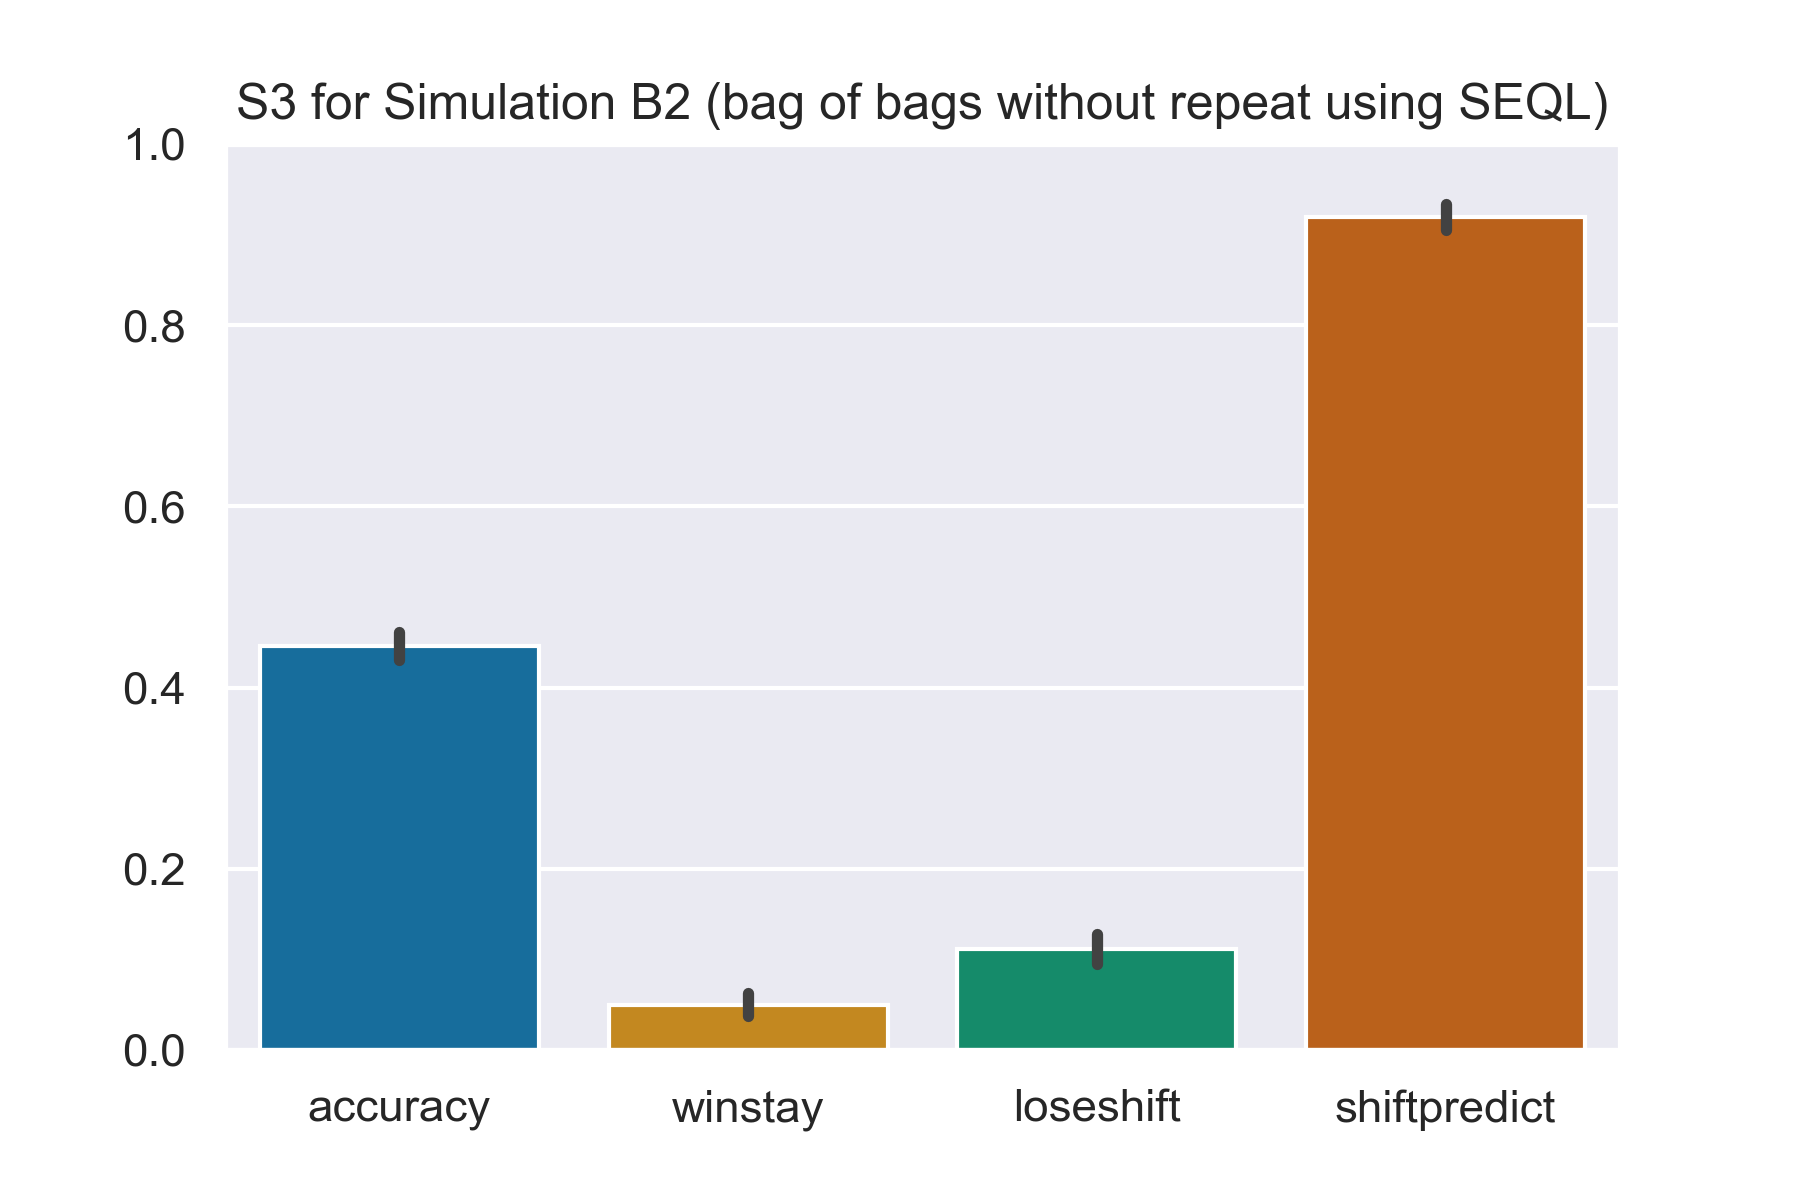
\includegraphics[width=0.9\linewidth, height=4cm]{plots/simB2_s3.png}
\label{fig:simB23}
\end{subfigure}
 
\caption{Numbers on y axis represent probability and is averaged across participants. From left to right; S1, S2 and S3. Upper row: Experiment B (bag of bags without repeat). Middle row: Simulation B1 (bag of bags without repeat using BQL). Lower row: Simulation B2 (bag of bags without repeat using SEQL)}
\label{fig:figure3}
\end{figure*}

\subsubsection{Experiment B: bag of bags without repeat}
In the bag of bags without repeat version of the task, participants had accuracy .73 (SD .34) for S1, .75 (SD .32) for S2 and .40 (SD .16) for S3. As we can see in Figure 3, participants show a similar pattern as in Experiment A for accuracy on S1 and S2, but here we see for S3 that participants show a strong tendency to pick another shape than the one they are currently seeing. In other words, they have spotted the pattern of shape shifts. This is supported by a majority answering positively about finding the pattern, a few even being able to describe precisely the ‘meta’ pattern that the bags would not repeat.

\subsubsection{Simulation B1: bag of bags without repeat (BQL)}

Average accuracy across simulated participants were .76 (SD .11) for S1, .85 (SD .12) for S2 and .03 (SD .05) for S3. This example simulation uses $\alpha = .61, \beta = .01, \gamma = .01$. No simulations were able to solve this task, i.e. show the same behaviour as the human participants, or manage the relaxed condition of more than .5 accuracy on S1 and S2 and more than .5 shift prediction on S3. Just as in Simulation A, they showed win-stay, lose-shift behaviour (Figure 3, middle row). 

\subsubsection{Simulation B2: bag of bags without repeat (SEQL)}

When enhancing the QL algorithm with states that include the position in each bag however, we do get behaviour that is qualitatively similar to the human data in Experiment B (Figure 3, bottom row). The particular simulation shown, using parameters $\alpha = .41, \beta = .01, \gamma = .01$, reveals almost optimal performance for several simulated participants. Average accuracy was for S1 .82 (SD .12), for S2 .81 (SD .14) and for S3 .45 (SD .08). Shift prediction was .18 (SD .12) on S1, .19 (SD .14) on S2 and .92 (SD .07) on S3.

\subsubsection{Experiment C: bag of bags}

Experiment C performance (not shown) was somewhere in-between Experiment A and B. Some individuals were able to spot the pattern, which can be seen in both the data and free text responses. But others were not able to, indicating a considerable degree of individual differences. Overall participants are generally accurate on S1 (mean .78, SD .29) and S2 (mean .79, SD .31) and showed a mean shift prediction of .59 (SD .30) on S3.

\subsubsection{Simulation C1: bag of bags (BQL)}

Overall, Simulation C1 (not shown) shows the same pattern again as Simulation B1, meaning no simulation solved the task. Average accuracy for artificial participants using $\alpha = .61, \beta = .01, \gamma = .21$, was .76 (SD .10) on S1, .85 (SD .11) on S2, while on S3 the shift prediction had mean .09 (SD .08).

\subsubsection{Simulation C2: bag of bags (SEQL)}

In Simulation C2 (not shown), as for Simulation B2, the SEQL model now has no issue learning the proper actions. Using $\alpha = .41, \beta = .01, \gamma = .01$ as our simulation example, accuracy for S1 was .80 (SD .15), for S2 .83 (SD .13) and for shift prediction on S3 .84 (SD .15). We see that on average S3 shift prediction is higher here than for the human participants in Experiment C (unpaired t-test; $t(122)=5.87, p=3.8\cdot10^{-8}$).

\subsubsection{Experiment D: random version (randomly seeded sequence)}

Just as in Experiment A, participants here fall back to win-stay, lose-shift. These results (not shown) are not as clearcut as in Experiment A; instead, we see the effect of random variation in the task sequence across participants. Some participants had sequences with higher frequencies of the longer runs (e.g. 6 or 9 repeats) of the same shape, and others had sequences that were closer to the bag of bags variants used in Experiment B or C. Accuracy was .71 (SD .23) for S1, .76 (SD .26) for S2 and .35 (SD .09) for S3. Winstay for S2 was .65 (SD .27) and .55 (SD .27) for S3. Shift prediction was .37 (SD .23) for S3, significantly lower than frequency of winstay for S3 (paired t-test; $t(38)=3.05, p=0.006$). Simulations of this experiment (not shown) are equivalent to simulation A for the BQL model.

\subsubsection{Simulation D: random version with SEQL}

In Simulation D (not shown), the results are generally unlike those of the human participants in Experiment D because they achieve a higher rate of shift prediction on S3, at a level similar to participants in Experiment C. For parameters $\alpha = .41, \beta = .01, \gamma = .01$ we get S1 accuracy .82 (SD .12), S2 accuracy .83 (SD .11) and S3 shift prediction .65 (SD .28).

\subsubsection{Summary} The main finding is the striking difference in human participants' ability to anticipate the state shifts in Experiment B in contrast to in Experiments A and D, and the role of enhanced state coding to allow SEQL to capture this behaviour. Experiment C was clearly easier (in terms of making the shift on S3) than the random version in Experiment A or D, but there seems to be a high degree of individual differences in performance. These results indicate that humans may enhance their representations of the world to solve tasks. If they do so, we also show how subtle changes in the task structure can impact the extent to which humans are able to create such representations. Additionally, our SPE version of RL is able to capture human behaviour in this task where explicit rewards are omitted.

\section{Discussion}

Our results suggest that humans are able to quickly employ suitable task representations to solve a task that requires them to do so. We also show that our SPE RL model can describe human behaviour in all three versions of the task, depending on the state representations used. This gives support for proposals suggesting a more general sensory prediction error view of RL. State representations are indeed important, and here we exemplify how model free RL can solve a task if it has access to appropriate state representations.

The most surprising aspect of these findings is the contrast between human performance across conditions: most of the humans quickly learn to adapt their state representations to solve the task in the bag of bags without repeat version. By contrast, many participants were not able to deploy the same enhanced state representations on the bag of bags variant and thus achieved prediction accuracies well below those of the simulations of the SEQL model. It seems participants unable to spot the pattern instead rely on a winstay-loseshift strategy, which can be seen as "good enough" as it is accurate in two thirds of the cases overall.

The shape sequence task thus looks promising for investigating previous proposals for how state representations are created and shaped through interaction with tasks \cite{Collins2013-cv,Eckstein2020-yi}. In such future work, we will also apply models such as the SPE proposed by Gardner et al. \citeyear{Gardner2018-vj} and episodic RL \cite{Gershman2017-ah}, as well as belief state representations \cite{Schuck2018-ik, Babayan2018-ix} to try to fit our shape sequence task data.

It is easy to imagine further variants of this task including adding explicit rewards for successful shape shift prediction, and using fMRI and/or EEG to identify neural substrates. The task can also be expanded in several ways, like including multiple dimensions, and such expansions may be needed to tease out differences in the models we plan to test. It is possible the approach of task sets as in \cite{Collins2013-cv} would fit our task by using the count of repeated shapes (first, second, third etc) as contexts which trigger differing task sets. Another view would be that our participants do not in fact employ different state representations here but instead learn compounded action sequences, as in the options framework \cite{Botvinick2009-bl}. Working memory also probably plays a part in the learning here \cite{Collins2012-kd}, perhaps especially contributing to the individual differences found for the bob version of the task.

Our SEQL version shows how relevant (if very simplified) state coding can enable MF algorithms to solve the task. However, to investigate the mechanism of how states and task structures are learned we might need artificial neural network approaches; for example where MF RL teaches a recurrent network the appropriate dynamics \cite{Botvinick2019-qf}. We can investigate whether these dynamics are similar to belief states \cite{Schuck2018-ik,Babayan2018-ix} that develop a task set representation \cite{Collins2013-cv} useful for RL and similar to that used in our SEQL model. In other words, once the statistical pattern of the transitions in the shape sequence task have been acquired, MF algorithms can perhaps use the emergent properties of the hidden layers to serve as an enhanced state representation.

In conclusion, our results show the value of this simple shape sequence task, especially for differentiating states with nominally identical stimuli, perhaps via rule sets depending on sequential context. Along with the successful simulations using SPE variants of basic QL, over a longer time-frame this might help us come closer to connecting the applied world of RL with the theoretical universe of predictive coding and free energy.


\section{Acknowledgments}

Thanks to reviewers for insightful feedback. Shringi Kumari and others for tips on visual design of experiment. All the participants. Coffee and whisky. This work was supported by the EPSRC Centre for Doctoral Training in Intelligent Games \& Games Intelligence (IGGI) [EP/L015846/1].



\bibliographystyle{apacite}

\setlength{\bibleftmargin}{.125in}
\setlength{\bibindent}{-\bibleftmargin}

\bibliography{references}


\end{document}
